% !Mode:: "TeX:UTF-8"
%!TEX program = xelatex
% 依据 2026-09-16 竞赛论文格式规范排版；上游类文件保持原样。
\documentclass[bwprint]{template/gmcmthesis}
\usepackage{template/official-format-2026}

\hypersetup{hidelinks}
\usepackage[framemethod=TikZ]{mdframed}
\usepackage{subfig}
\usepackage{placeins}
\AddToHook{env/thebibliography/before}{\FloatBarrier}
\usepackage{siunitx}
\usepackage{colortbl}
\usepackage[noend]{algpseudocode}
\usepackage{algorithmicx,algorithm}
\usepackage{amsmath,amssymb,booktabs,graphicx}
\captionsetup[figure]{format=plain,justification=centering,singlelinecheck=false}
\newcommand{\formulaname}[1]{\par\smallskip\noindent{\songti\zihao{-4}#1}\par\nobreak}
\graphicspath{{./}{figures/q1-mixture-scale/}{figures/q1-conflict-resolution/}{figures/q1-critic-topsis/nature-v1/}{template/figures/}}
% 统一符号、命令和术语。新增命令先在这里登记。
\newcommand{\R}{\mathbb{R}}
\newcommand{\E}{\mathbb{E}}
\newcommand{\argmin}{\operatorname*{arg\,min}}

\numberwithin{equation}{section}
\counterwithin{figure}{section}
\counterwithin{table}{section}

\title{数据质量评价、冲突消解与训练配比规模修正}

\floatname{algorithm}{算法}
\renewcommand{\algorithmicrequire}{\textbf{输入:}}
\renewcommand{\algorithmicensure}{\textbf{输出:}}

\begin{document}

\maketitle
\begin{abstract}
本文研究多源文本质量评价、质量信号冲突及训练领域配比对语言模型 Loss 的影响。首先以 A1 拟合集固定归一化边界和 CRITIC 权重，用加权距离 TOPSIS 对 261,086 条去重记录评分；随后将通用指标归并为五维，以分位阈值标记候选冲突并构造有限补偿评分；最后用 ilr-Ridge 建立配比与 13 个验证目标 Loss 的关系，以同配方跨规模差分校准规模偏差。全量语料均分为 54.2323，较 A1 的 60.9471 低 6.7149 分，主要由领域构成变化驱动；全量候选冲突率为 34.5966\%。二阶配比模型将 1M 同尺度 RMSE 从 0.3464 降至 0.2840；配方条件规模修正将 1B 回顾评价 RMSE 从 2.6963 降至 0.6252。本文的模型构造将冻结评价标尺、有限补偿与配方条件规模校准衔接；高规模 Loss 来自给定估算，质量代理亦未获得独立验证，因此不据此断言最优训练配方。
\par
\keywords{数据质量评价\quad CRITIC--TOPSIS\quad 冲突消解\quad 有限补偿\quad 配比效应\quad 规模修正}
\end{abstract}
\pagestyle{plain}

%% 可直接由仓库 paper/main.tex 通过 %% 可直接由仓库 paper/main.tex 通过 %% 可直接由仓库 paper/main.tex 通过 \input{sections/q1-quality-evaluation.tex} 引入。
%% 依照 paper/template/gmcmthesis.cls 的章节、公式、图形和 booktabs 表格规范编写。
\section{问题一：数据质量评价与基础评分}

\subsection{问题分析与总体框架}
本小问的目标是将抽样集与扩展集中的多源文本质量信号统一到同一评价尺度，形成可解释、可追溯的质量分数。评价对象包括抽样集 $A_1$、扩展集 $A_2$ 和扩展集 $A_3$ 的全部记录：$A_1$ 包含 $51{,}230$ 条记录，$A_2$ 包含 $17{,}523$ 条记录，$A_3$ 包含 $203{,}752$ 条记录。合并后先按记录指纹去重，得到 $261{,}086$ 条有效记录，去重前后删除 $11{,}419$ 条重复记录。模型流程为“全量合并与去重—指标方向统一—稳健归一化—CRITIC 客观赋权—加权距离 TOPSIS 评分—样本、领域和语料级聚合—抽样集对照”。

\begin{figure}[htbp]
  \centering
  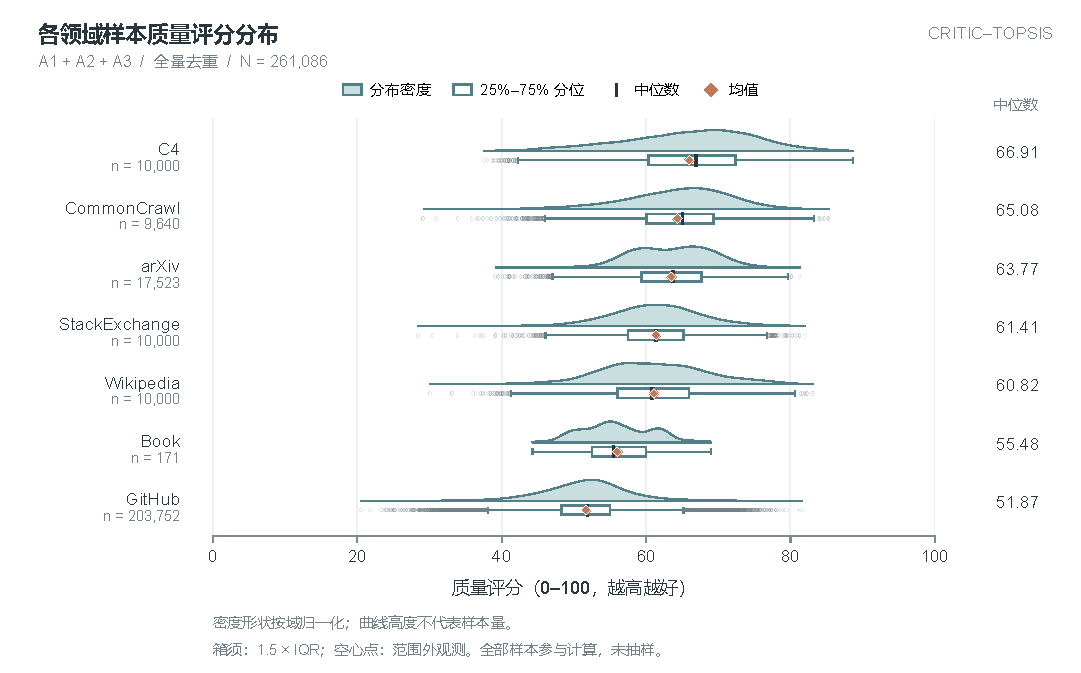
\includegraphics[width=\linewidth,height=0.42\textheight,keepaspectratio]{figures/q1-critic-topsis/nature-v1/figure01_domain_distribution_nature.pdf}
  \caption{领域质量分布图}
  \label{fig:q1-nature-01}
\end{figure}

\subsection{数据对象与预处理}
第 $i$ 条记录具有 16 维原始质量指标向量。指标覆盖语言形式、可读性、内容质量、教育性、事实性、知识覆盖与重复性等维度，其中句末标点率、cleanliness、no-ad、readability、fluency、unique words、QuRating education、writing、FineWeb education、factual、Books、Math 和 Wikipedia 为正向指标；无字母词比例、最高频二元词组占比和最高频三元词组占比为负向指标。负向指标较大时通常意味着文本更可能由符号、模板或高频短语主导，因此需要反向处理。
\formulaname{原始质量指标向量公式}
\begin{equation}
 \boldsymbol{x}_i=(x_{i1},\ldots,x_{i16}).
 \label{eq:q1-indicator-vector}
\end{equation}

正向与负向指标集合分别记为 $\mathcal P$、$\mathcal N$，两者互不相交且覆盖全部 16 个指标。方向统一后的指标定义如下。
\formulaname{指标方向统一公式}
\begin{equation}
 \widetilde{x}_{ij}=\begin{cases}
 x_{ij}, & j\in\mathcal{P},\\
 -x_{ij}, & j\in\mathcal{N}
 \end{cases}
 \label{eq:q1-direction-unification}
\end{equation}
随后使用方向统一值的 $A_1$ 拟合 $1\%$ 和 $99\%$ 分位点作为稳健边界；记边界为 $l_j$ 和 $u_j$，则统一为“越高越好”的稳健归一化形式。这里 $\operatorname{clip}(t,0,1)$ 表示将 $t$ 截断至 $[0,1]$。
\formulaname{稳健归一化公式}
\begin{equation}
 z_{ij}=\operatorname{clip}\left(\frac{\widetilde{x}_{ij}-l_j}{u_j-l_j},0,1\right).
 \label{eq:q1-robust-normalization}
\end{equation}
扩展集只使用 $A_1$ 的边界，不重新拟合分位点，从而保证 $A_1$、$A_2$ 和 $A_3$ 的分数具有可比性。归一化后检查缺失值、无穷值、越界值和重复指纹，并保留每条记录的来源集、领域标签和质量分数，供后续聚合与审计。

\begin{figure}[htbp]
  \centering
  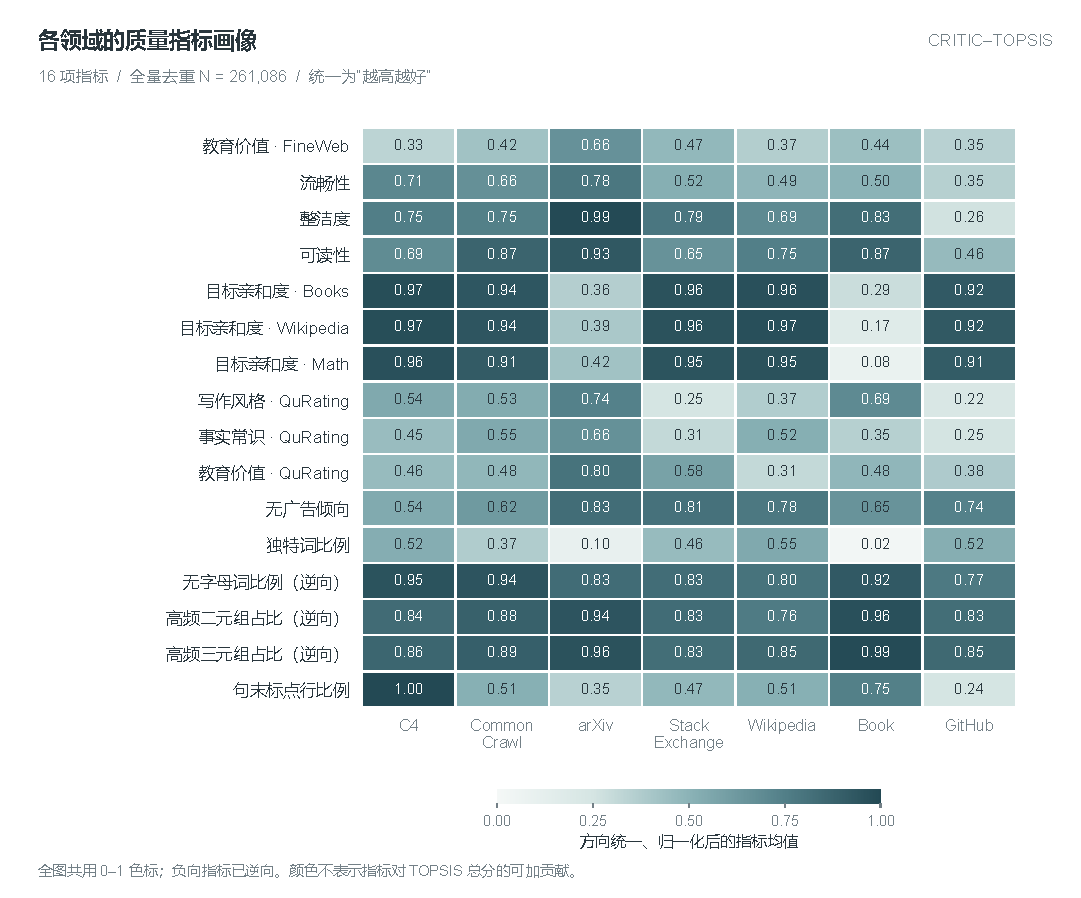
\includegraphics[width=\linewidth,height=0.42\textheight,keepaspectratio]{figures/q1-critic-topsis/nature-v1/figure02_indicator_heatmap_nature.pdf}
  \caption{领域质量指标画像图}
  \label{fig:q1-nature-02}
\end{figure}

\subsection{CRITIC 客观赋权}
为避免人为指定权重，采用 CRITIC 方法同时利用指标的离散程度和冲突程度。设归一化矩阵为 $Z$，其元素为 $z_{ij}$；第 $j$ 个指标的标准差为 $\sigma_j$，与第 $k$ 个指标的 Pearson 相关系数为 $r_{jk}$。
\formulaname{CRITIC 信息量公式}
\begin{equation}
 I_j=\sigma_j\sum_{k=1}^{16}(1-r_{jk}).
 \label{eq:q1-critic-information}
\end{equation}
\formulaname{CRITIC 权重公式}
\begin{equation}
 w_j=\frac{I_j}{\sum_{m=1}^{16}I_m}.
 \label{eq:q1-critic}
\end{equation}
其中，$\sigma_j$ 反映指标对样本的区分能力，$1-r_{jk}$ 反映该指标与其他指标的信息差异。由 $A_1$ 的拟合集计算权重并固定应用于 $A_1$ 留出集及 $A_2$、$A_3$，既防止扩展集的分布变化改变权重，又保证外推比较的可重复性。最终权重最高的指标为句末标点率（$8.9093\%$）、cleanliness（$8.0008\%$）和 no-ad（$7.7530\%$）；三个负向词组指标合计权重为 $16.5784\%$。

\begin{figure}[htbp]
  \centering
  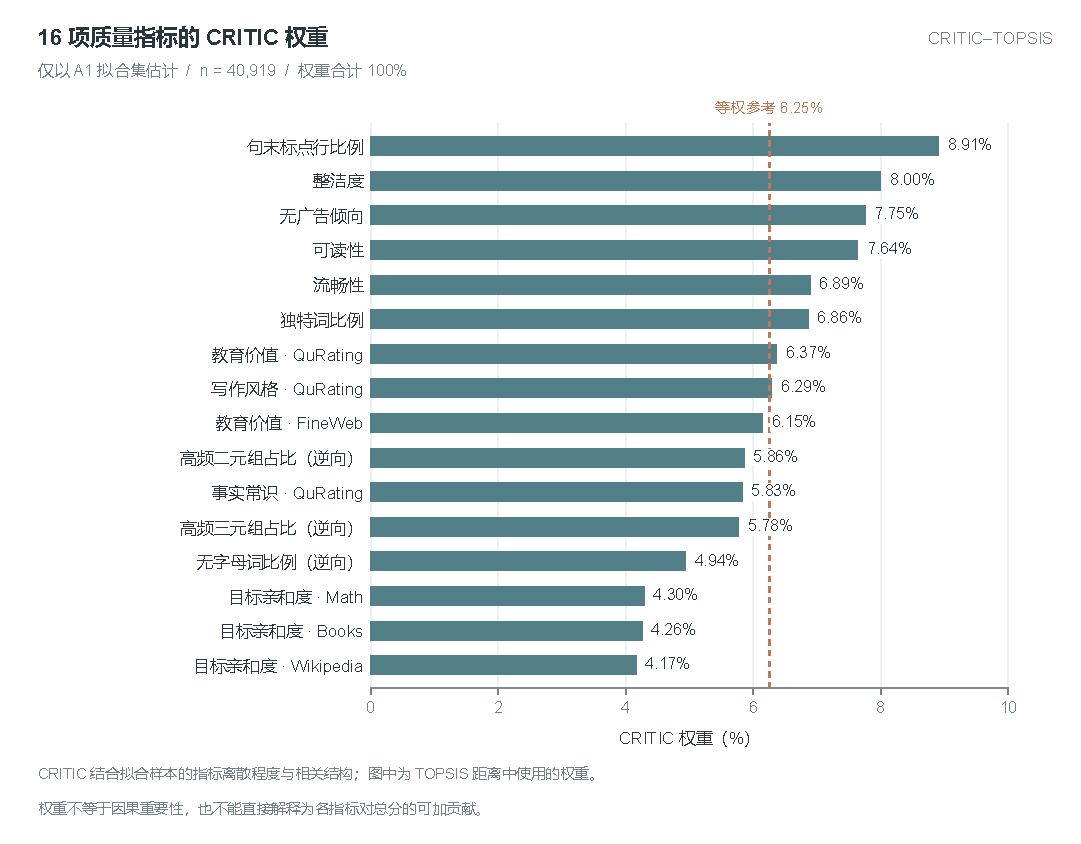
\includegraphics[width=\linewidth,height=0.42\textheight,keepaspectratio]{figures/q1-critic-topsis/nature-v1/figure05_critic_weights_nature.pdf}
  \caption{质量指标权重图}
  \label{fig:q1-nature-05}
\end{figure}

\subsection{加权距离 TOPSIS 评分}
以取值全为 1 的正向理想点 $\boldsymbol{z}^{+}$ 和取值全为 0 的负向理想点 $\boldsymbol{z}^{-}$ 为参照，计算第 $i$ 条记录到两类理想点的加权欧氏距离。
\formulaname{正理想点距离公式}
\begin{equation}
 D_i^{+}=\sqrt{\sum_{j=1}^{16}w_j(1-z_{ij})^2}.
 \label{eq:q1-topsis-positive-distance}
\end{equation}
\formulaname{负理想点距离公式}
\begin{equation}
 D_i^{-}=\sqrt{\sum_{j=1}^{16}w_jz_{ij}^2}.
 \label{eq:q1-topsis-distance}
\end{equation}
样本级质量分数定义如下，其取值在 $[0,100]$。
\formulaname{样本质量分数公式}
\begin{equation}
 Q_i=100\times\frac{D_i^{-}}{D_i^{+}+D_i^{-}}.
 \label{eq:q1-topsis-score}
\end{equation}
因此，$Q_i$ 越大表示该记录越接近理想高质量点。该分数回答的是“单条文本在 16 个统一方向质量信号下的综合质量水平”，而非某个单一指标的原始测量值。

\begin{figure}[htbp]
  \centering
  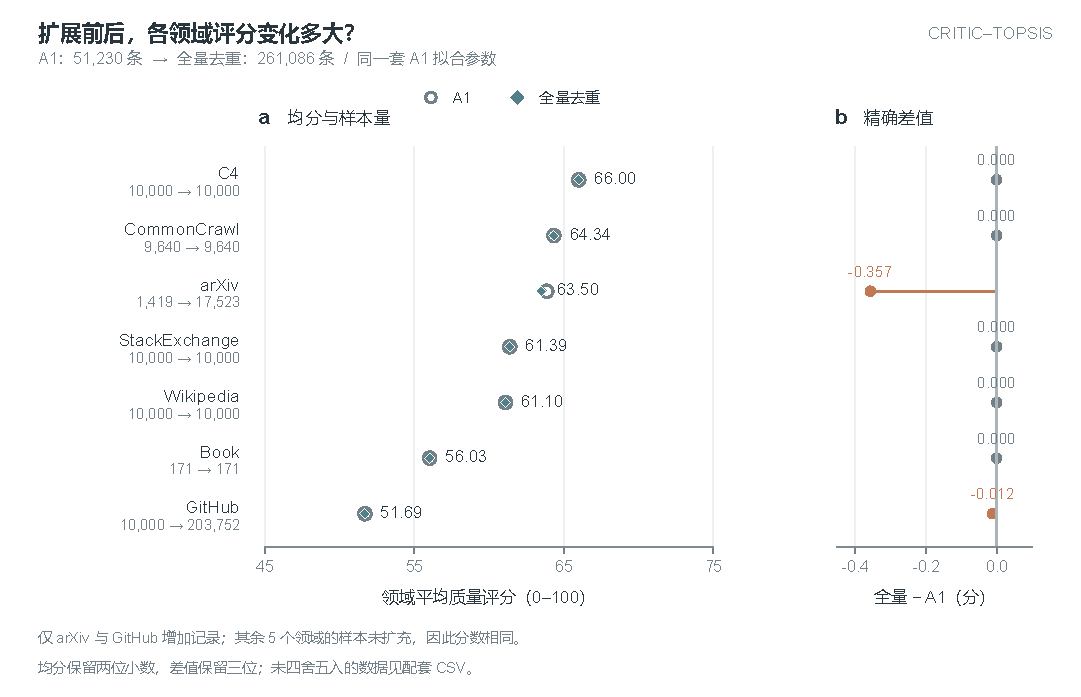
\includegraphics[width=\linewidth,height=0.42\textheight,keepaspectratio]{figures/q1-critic-topsis/nature-v1/figure03_A1_full_comparison_nature.pdf}
  \caption{领域均分对照图}
  \label{fig:q1-nature-03}
\end{figure}

\subsection{从样本级到领域级和语料级的聚合}
对领域 $g$ 的记录集合 $\mathcal{I}_g$，采用样本数加权的均值聚合。
\formulaname{领域质量均值公式}
\begin{equation}
 Q_g=\frac{1}{|\mathcal{I}_g|}\sum_{i\in\mathcal{I}_g}Q_i.
 \label{eq:q1-domain-aggregation}
\end{equation}
语料级分数同样由全体记录的样本均值给出。这种聚合保留了每条记录的等贡献原则，并能将域级差异与域规模分离：域均值反映质量，域记录数反映组成。若需降低极端值影响，可在附录中同时报告中位数和四分位距，但主结果使用均值以便与全量语料平均质量一致。
\formulaname{语料质量均值公式}
\begin{equation}
 Q_{\mathrm{corpus}}=\frac{1}{N}\sum_{i=1}^{N}Q_i.
 \label{eq:q1-corpus-aggregation}
\end{equation}

\begin{figure}[htbp]
  \centering
  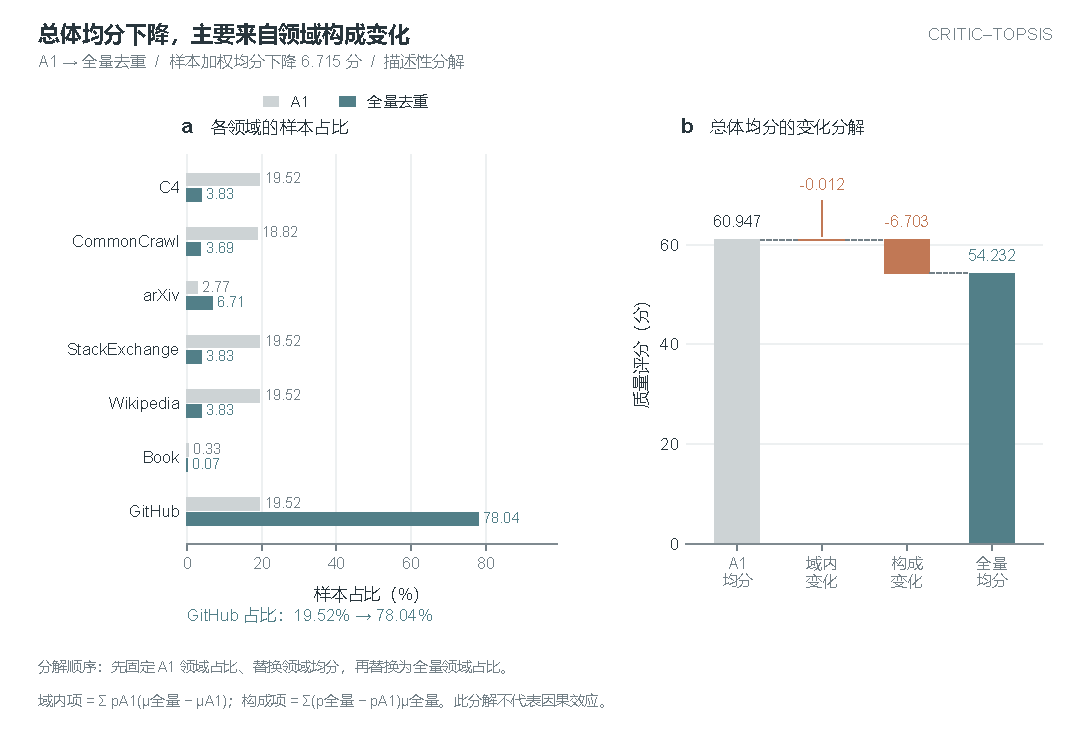
\includegraphics[width=\linewidth,height=0.42\textheight,keepaspectratio]{figures/q1-critic-topsis/nature-v1/figure04_composition_decomposition_nature.pdf}
  \caption{领域构成分解图}
  \label{fig:q1-nature-04}
\end{figure}

\subsection{全量结果与抽样集对照}
$A_1$ 语料级平均分为 $60.9471$，全量去重语料平均分为 $54.2323$，整体下降 $6.7149$ 分。按领域对照时，arxiv 从 $63.8624$ 变为 $63.5050$，下降 $0.3574$ 分；github 从 $51.7014$ 变为 $51.6893$，下降 $0.0121$ 分；book、c4、commoncrawl、stackexchange 和 wikipedia 的领域均值保持不变或仅发生四舍五入范围内的变化。由此可见，全量平均分下降主要来自领域组成变化，而不是各领域内部质量普遍恶化。GitHub 在 $A_1$ 中约占 $19.52\%$，在全量去重语料中约占 $78.04\%$，其较低的领域均值显著拉低了全量语料级分数。

\begin{table}[htbp]
  \centering
  \caption{$A_1$ 与全量去重语料的领域级质量分数对照}
  \label{tab:q1-domain-score}

  \renewcommand{\arraystretch}{1.15}
  \begin{tabular}{lrrrr}
    \toprule
    领域 & $A_1$ 均值 & 全量均值 & 变化 & 全量占比 \\
    \midrule
    arxiv & 63.8624 & 63.5050 & -0.3574 & 6.71\% \\
    book & 56.0325 & 56.0325 & 0.0000 & 0.07\% \\
    c4 & 66.0021 & 66.0021 & 0.0000 & 3.83\% \\
    commoncrawl & 64.3357 & 64.3357 & 0.0000 & 3.69\% \\
    github & 51.7014 & 51.6893 & -0.0121 & 78.04\% \\
    stackexchange & 61.3879 & 61.3879 & 0.0000 & 3.83\% \\
    wikipedia & 61.1009 & 61.1009 & 0.0000 & 3.83\% \\
    \addlinespace[0.5ex]
    语料级均值 & 60.9471 & 54.2323 & -6.7149 & 100.00\% \\
    \bottomrule
  \end{tabular}
\end{table}

\subsection{稳健性与适用边界}
将 CRITIC--TOPSIS 结果与等权加权、删除 DSIR 以及删除三个负向词组指标的敏感性方案比较。CRITIC 加权和等权结果的 Spearman 相关系数为 $0.9877$，CRITIC 结果与删除 DSIR 的结果相关系数为 $0.9860$，与删除三个负向指标的结果相关系数为 $0.9674$。在删除负向指标的方案中，平均名次变化为 $4.79$ 个百分点，约 $2.78\%$ 的记录名次变化超过 $20$ 个百分点，说明重复性指标虽不是唯一质量依据，但对尾部样本的排序具有实质影响。这里的敏感性分析用于检查第一小问质量评分对建模选择的稳定性；它不等同于问题一后续小问中对指标冲突的独立量化。

\begin{figure}[htbp]
  \centering
  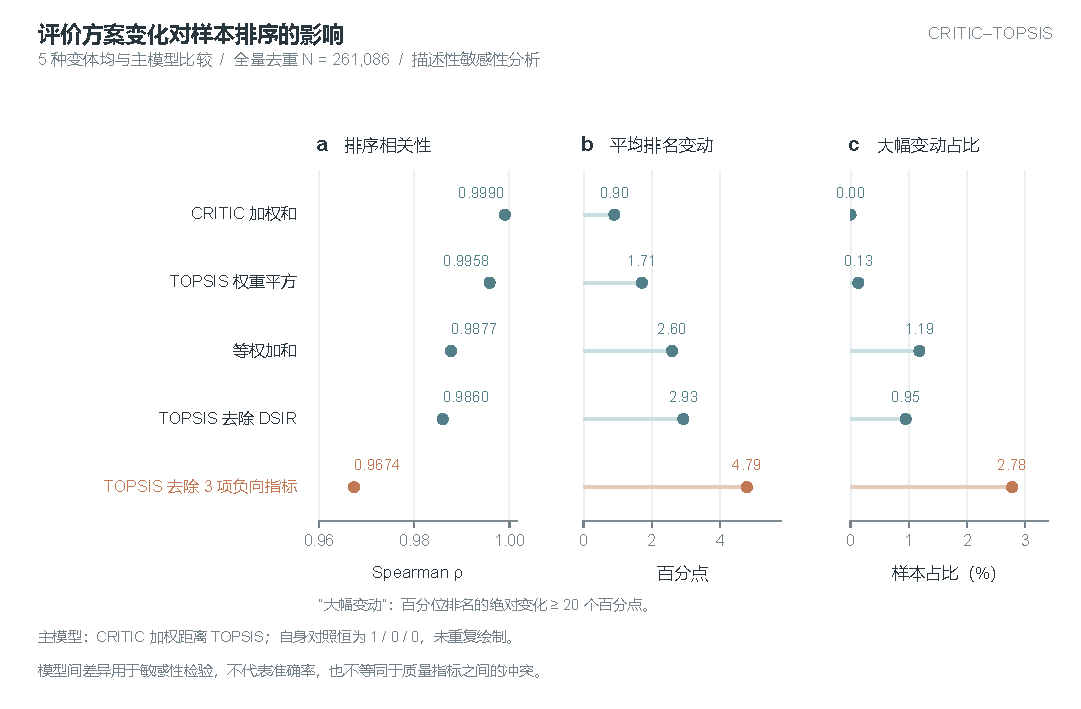
\includegraphics[width=\linewidth,height=0.42\textheight,keepaspectratio]{figures/q1-critic-topsis/nature-v1/figure06_model_sensitivity_nature.pdf}
  \caption{评分排序敏感性图}
  \label{fig:q1-nature-06}
\end{figure}

\subsection{小结}
本小问形成了一个可复算的全量质量评价链条：以 $A_1$ 的稳健边界和 CRITIC 权重建立统一标尺，以加权距离 TOPSIS 输出样本级质量分数，再按记录均值聚合为领域级和语料级分数。结果表明，$A_1$ 与扩展后的全量语料在领域内部质量上总体稳定，语料级平均分的主要变化由领域配比改变所致。该结论为后续质量冲突识别和数据配比优化提供可追溯的基线。
 引入。
%% 依照 paper/template/gmcmthesis.cls 的章节、公式、图形和 booktabs 表格规范编写。
\section{问题一：数据质量评价与基础评分}

\subsection{问题分析与总体框架}
本小问的目标是将抽样集与扩展集中的多源文本质量信号统一到同一评价尺度，形成可解释、可追溯的质量分数。评价对象包括抽样集 $A_1$、扩展集 $A_2$ 和扩展集 $A_3$ 的全部记录：$A_1$ 包含 $51{,}230$ 条记录，$A_2$ 包含 $17{,}523$ 条记录，$A_3$ 包含 $203{,}752$ 条记录。合并后先按记录指纹去重，得到 $261{,}086$ 条有效记录，去重前后删除 $11{,}419$ 条重复记录。模型流程为“全量合并与去重—指标方向统一—稳健归一化—CRITIC 客观赋权—加权距离 TOPSIS 评分—样本、领域和语料级聚合—抽样集对照”。

\begin{figure}[htbp]
  \centering
  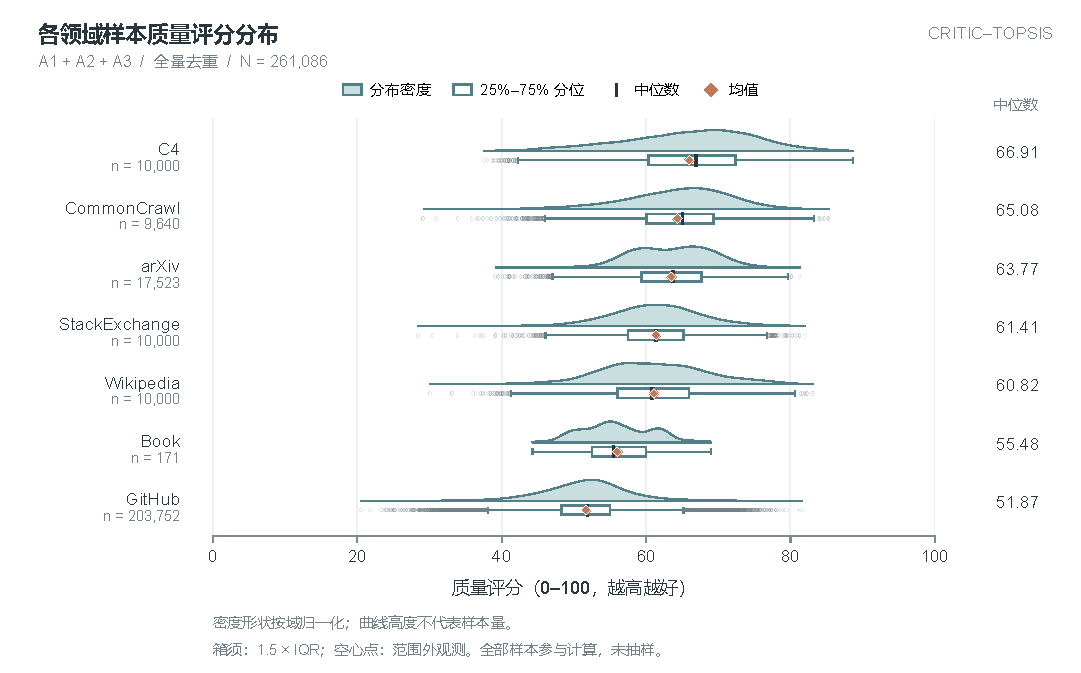
\includegraphics[width=\linewidth,height=0.42\textheight,keepaspectratio]{figures/q1-critic-topsis/nature-v1/figure01_domain_distribution_nature.pdf}
  \caption{领域质量分布图}
  \label{fig:q1-nature-01}
\end{figure}

\subsection{数据对象与预处理}
第 $i$ 条记录具有 16 维原始质量指标向量。指标覆盖语言形式、可读性、内容质量、教育性、事实性、知识覆盖与重复性等维度，其中句末标点率、cleanliness、no-ad、readability、fluency、unique words、QuRating education、writing、FineWeb education、factual、Books、Math 和 Wikipedia 为正向指标；无字母词比例、最高频二元词组占比和最高频三元词组占比为负向指标。负向指标较大时通常意味着文本更可能由符号、模板或高频短语主导，因此需要反向处理。
\formulaname{原始质量指标向量公式}
\begin{equation}
 \boldsymbol{x}_i=(x_{i1},\ldots,x_{i16}).
 \label{eq:q1-indicator-vector}
\end{equation}

正向与负向指标集合分别记为 $\mathcal P$、$\mathcal N$，两者互不相交且覆盖全部 16 个指标。方向统一后的指标定义如下。
\formulaname{指标方向统一公式}
\begin{equation}
 \widetilde{x}_{ij}=\begin{cases}
 x_{ij}, & j\in\mathcal{P},\\
 -x_{ij}, & j\in\mathcal{N}
 \end{cases}
 \label{eq:q1-direction-unification}
\end{equation}
随后使用方向统一值的 $A_1$ 拟合 $1\%$ 和 $99\%$ 分位点作为稳健边界；记边界为 $l_j$ 和 $u_j$，则统一为“越高越好”的稳健归一化形式。这里 $\operatorname{clip}(t,0,1)$ 表示将 $t$ 截断至 $[0,1]$。
\formulaname{稳健归一化公式}
\begin{equation}
 z_{ij}=\operatorname{clip}\left(\frac{\widetilde{x}_{ij}-l_j}{u_j-l_j},0,1\right).
 \label{eq:q1-robust-normalization}
\end{equation}
扩展集只使用 $A_1$ 的边界，不重新拟合分位点，从而保证 $A_1$、$A_2$ 和 $A_3$ 的分数具有可比性。归一化后检查缺失值、无穷值、越界值和重复指纹，并保留每条记录的来源集、领域标签和质量分数，供后续聚合与审计。

\begin{figure}[htbp]
  \centering
  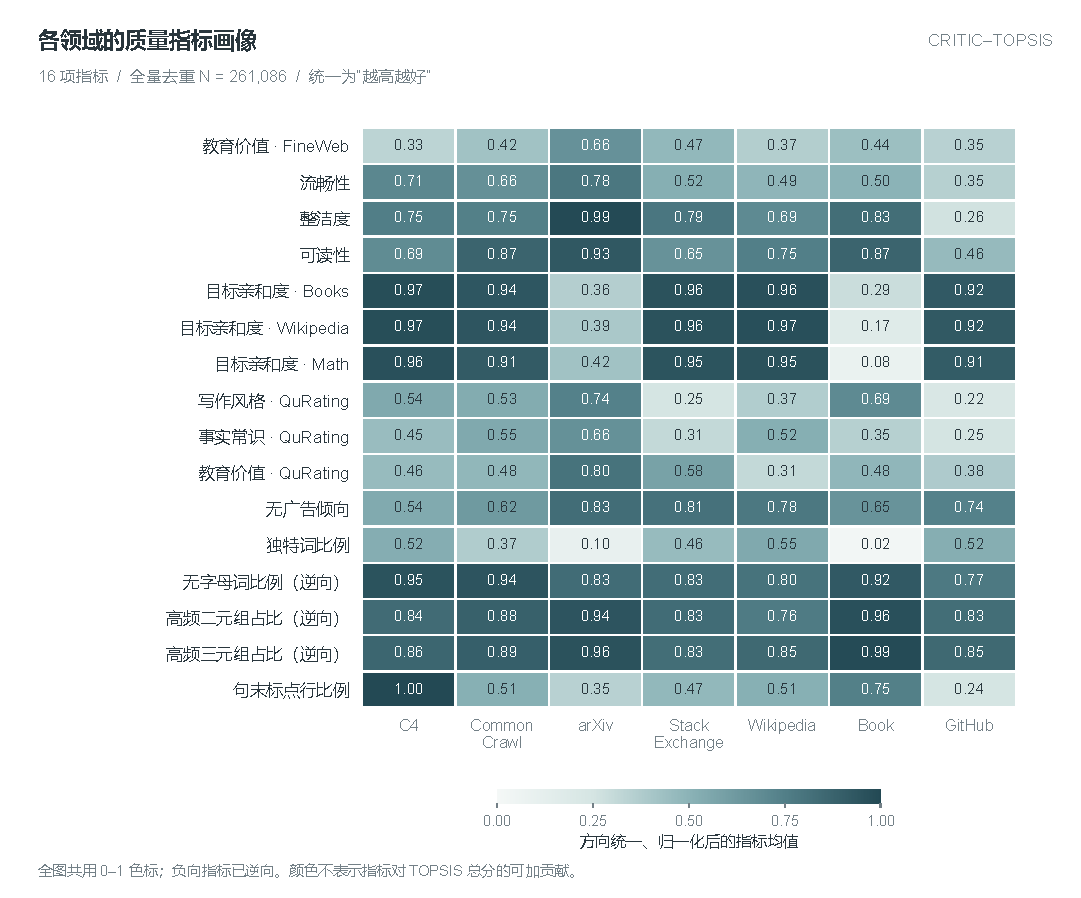
\includegraphics[width=\linewidth,height=0.42\textheight,keepaspectratio]{figures/q1-critic-topsis/nature-v1/figure02_indicator_heatmap_nature.pdf}
  \caption{领域质量指标画像图}
  \label{fig:q1-nature-02}
\end{figure}

\subsection{CRITIC 客观赋权}
为避免人为指定权重，采用 CRITIC 方法同时利用指标的离散程度和冲突程度。设归一化矩阵为 $Z$，其元素为 $z_{ij}$；第 $j$ 个指标的标准差为 $\sigma_j$，与第 $k$ 个指标的 Pearson 相关系数为 $r_{jk}$。
\formulaname{CRITIC 信息量公式}
\begin{equation}
 I_j=\sigma_j\sum_{k=1}^{16}(1-r_{jk}).
 \label{eq:q1-critic-information}
\end{equation}
\formulaname{CRITIC 权重公式}
\begin{equation}
 w_j=\frac{I_j}{\sum_{m=1}^{16}I_m}.
 \label{eq:q1-critic}
\end{equation}
其中，$\sigma_j$ 反映指标对样本的区分能力，$1-r_{jk}$ 反映该指标与其他指标的信息差异。由 $A_1$ 的拟合集计算权重并固定应用于 $A_1$ 留出集及 $A_2$、$A_3$，既防止扩展集的分布变化改变权重，又保证外推比较的可重复性。最终权重最高的指标为句末标点率（$8.9093\%$）、cleanliness（$8.0008\%$）和 no-ad（$7.7530\%$）；三个负向词组指标合计权重为 $16.5784\%$。

\begin{figure}[htbp]
  \centering
  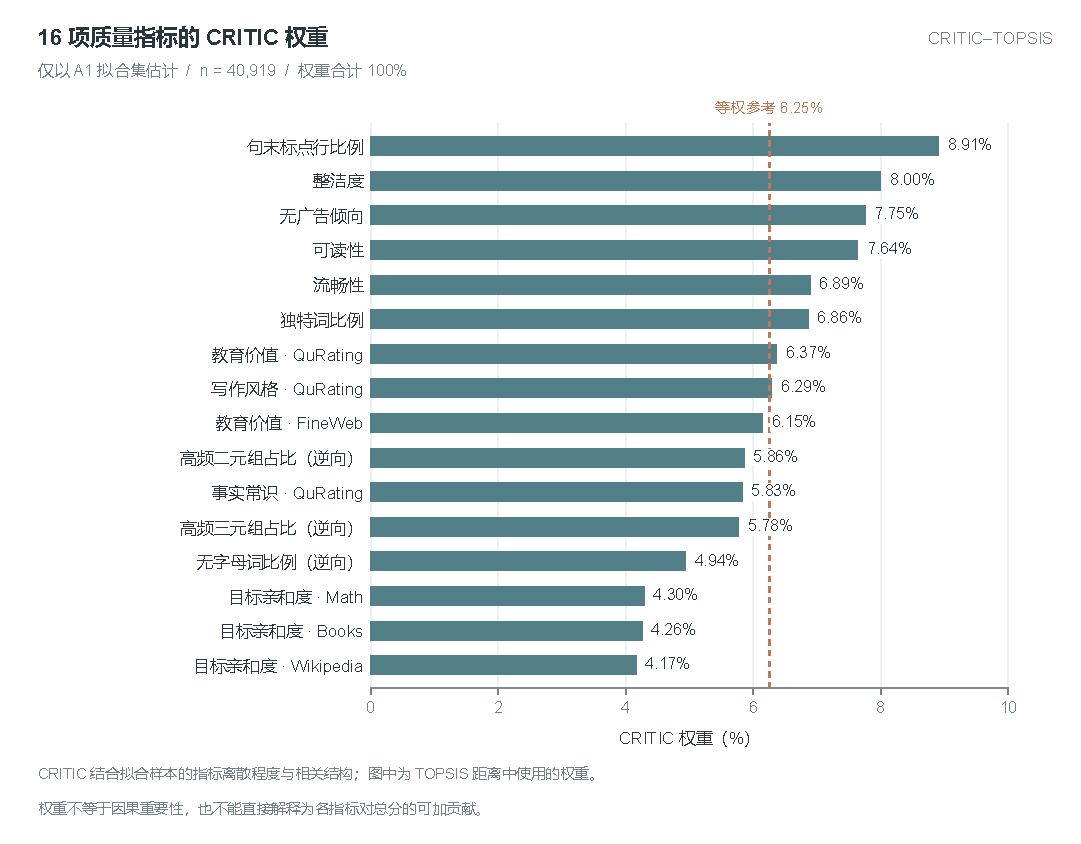
\includegraphics[width=\linewidth,height=0.42\textheight,keepaspectratio]{figures/q1-critic-topsis/nature-v1/figure05_critic_weights_nature.pdf}
  \caption{质量指标权重图}
  \label{fig:q1-nature-05}
\end{figure}

\subsection{加权距离 TOPSIS 评分}
以取值全为 1 的正向理想点 $\boldsymbol{z}^{+}$ 和取值全为 0 的负向理想点 $\boldsymbol{z}^{-}$ 为参照，计算第 $i$ 条记录到两类理想点的加权欧氏距离。
\formulaname{正理想点距离公式}
\begin{equation}
 D_i^{+}=\sqrt{\sum_{j=1}^{16}w_j(1-z_{ij})^2}.
 \label{eq:q1-topsis-positive-distance}
\end{equation}
\formulaname{负理想点距离公式}
\begin{equation}
 D_i^{-}=\sqrt{\sum_{j=1}^{16}w_jz_{ij}^2}.
 \label{eq:q1-topsis-distance}
\end{equation}
样本级质量分数定义如下，其取值在 $[0,100]$。
\formulaname{样本质量分数公式}
\begin{equation}
 Q_i=100\times\frac{D_i^{-}}{D_i^{+}+D_i^{-}}.
 \label{eq:q1-topsis-score}
\end{equation}
因此，$Q_i$ 越大表示该记录越接近理想高质量点。该分数回答的是“单条文本在 16 个统一方向质量信号下的综合质量水平”，而非某个单一指标的原始测量值。

\begin{figure}[htbp]
  \centering
  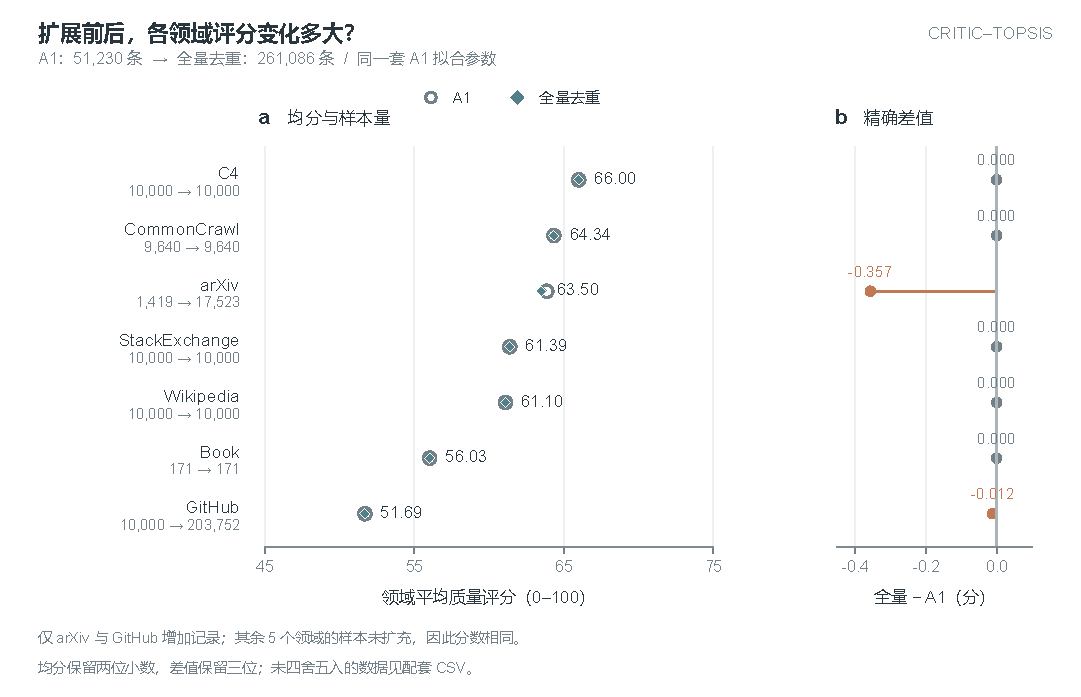
\includegraphics[width=\linewidth,height=0.42\textheight,keepaspectratio]{figures/q1-critic-topsis/nature-v1/figure03_A1_full_comparison_nature.pdf}
  \caption{领域均分对照图}
  \label{fig:q1-nature-03}
\end{figure}

\subsection{从样本级到领域级和语料级的聚合}
对领域 $g$ 的记录集合 $\mathcal{I}_g$，采用样本数加权的均值聚合。
\formulaname{领域质量均值公式}
\begin{equation}
 Q_g=\frac{1}{|\mathcal{I}_g|}\sum_{i\in\mathcal{I}_g}Q_i.
 \label{eq:q1-domain-aggregation}
\end{equation}
语料级分数同样由全体记录的样本均值给出。这种聚合保留了每条记录的等贡献原则，并能将域级差异与域规模分离：域均值反映质量，域记录数反映组成。若需降低极端值影响，可在附录中同时报告中位数和四分位距，但主结果使用均值以便与全量语料平均质量一致。
\formulaname{语料质量均值公式}
\begin{equation}
 Q_{\mathrm{corpus}}=\frac{1}{N}\sum_{i=1}^{N}Q_i.
 \label{eq:q1-corpus-aggregation}
\end{equation}

\begin{figure}[htbp]
  \centering
  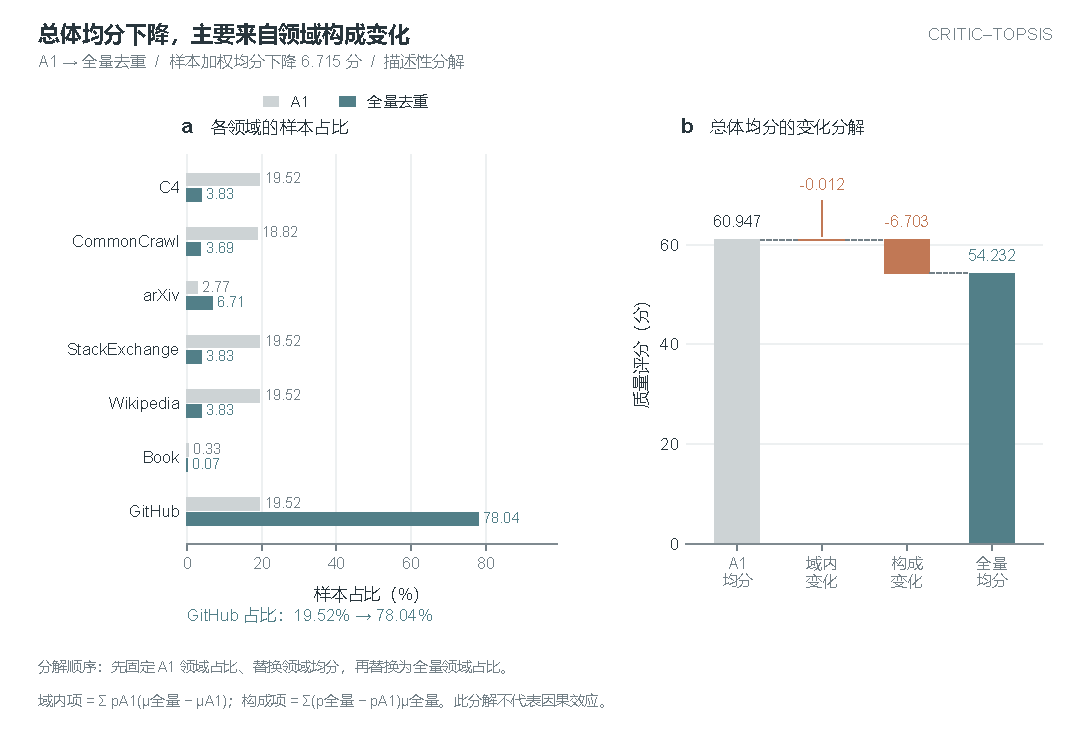
\includegraphics[width=\linewidth,height=0.42\textheight,keepaspectratio]{figures/q1-critic-topsis/nature-v1/figure04_composition_decomposition_nature.pdf}
  \caption{领域构成分解图}
  \label{fig:q1-nature-04}
\end{figure}

\subsection{全量结果与抽样集对照}
$A_1$ 语料级平均分为 $60.9471$，全量去重语料平均分为 $54.2323$，整体下降 $6.7149$ 分。按领域对照时，arxiv 从 $63.8624$ 变为 $63.5050$，下降 $0.3574$ 分；github 从 $51.7014$ 变为 $51.6893$，下降 $0.0121$ 分；book、c4、commoncrawl、stackexchange 和 wikipedia 的领域均值保持不变或仅发生四舍五入范围内的变化。由此可见，全量平均分下降主要来自领域组成变化，而不是各领域内部质量普遍恶化。GitHub 在 $A_1$ 中约占 $19.52\%$，在全量去重语料中约占 $78.04\%$，其较低的领域均值显著拉低了全量语料级分数。

\begin{table}[htbp]
  \centering
  \caption{$A_1$ 与全量去重语料的领域级质量分数对照}
  \label{tab:q1-domain-score}

  \renewcommand{\arraystretch}{1.15}
  \begin{tabular}{lrrrr}
    \toprule
    领域 & $A_1$ 均值 & 全量均值 & 变化 & 全量占比 \\
    \midrule
    arxiv & 63.8624 & 63.5050 & -0.3574 & 6.71\% \\
    book & 56.0325 & 56.0325 & 0.0000 & 0.07\% \\
    c4 & 66.0021 & 66.0021 & 0.0000 & 3.83\% \\
    commoncrawl & 64.3357 & 64.3357 & 0.0000 & 3.69\% \\
    github & 51.7014 & 51.6893 & -0.0121 & 78.04\% \\
    stackexchange & 61.3879 & 61.3879 & 0.0000 & 3.83\% \\
    wikipedia & 61.1009 & 61.1009 & 0.0000 & 3.83\% \\
    \addlinespace[0.5ex]
    语料级均值 & 60.9471 & 54.2323 & -6.7149 & 100.00\% \\
    \bottomrule
  \end{tabular}
\end{table}

\subsection{稳健性与适用边界}
将 CRITIC--TOPSIS 结果与等权加权、删除 DSIR 以及删除三个负向词组指标的敏感性方案比较。CRITIC 加权和等权结果的 Spearman 相关系数为 $0.9877$，CRITIC 结果与删除 DSIR 的结果相关系数为 $0.9860$，与删除三个负向指标的结果相关系数为 $0.9674$。在删除负向指标的方案中，平均名次变化为 $4.79$ 个百分点，约 $2.78\%$ 的记录名次变化超过 $20$ 个百分点，说明重复性指标虽不是唯一质量依据，但对尾部样本的排序具有实质影响。这里的敏感性分析用于检查第一小问质量评分对建模选择的稳定性；它不等同于问题一后续小问中对指标冲突的独立量化。

\begin{figure}[htbp]
  \centering
  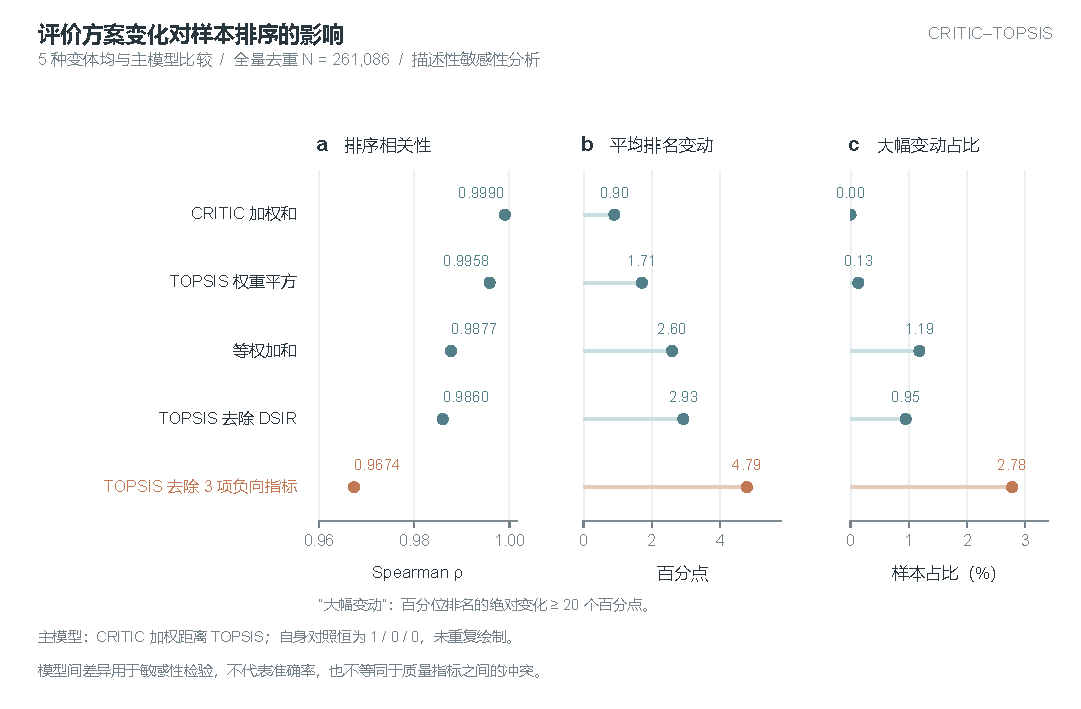
\includegraphics[width=\linewidth,height=0.42\textheight,keepaspectratio]{figures/q1-critic-topsis/nature-v1/figure06_model_sensitivity_nature.pdf}
  \caption{评分排序敏感性图}
  \label{fig:q1-nature-06}
\end{figure}

\subsection{小结}
本小问形成了一个可复算的全量质量评价链条：以 $A_1$ 的稳健边界和 CRITIC 权重建立统一标尺，以加权距离 TOPSIS 输出样本级质量分数，再按记录均值聚合为领域级和语料级分数。结果表明，$A_1$ 与扩展后的全量语料在领域内部质量上总体稳定，语料级平均分的主要变化由领域配比改变所致。该结论为后续质量冲突识别和数据配比优化提供可追溯的基线。
 引入。
%% 依照 paper/template/gmcmthesis.cls 的章节、公式、图形和 booktabs 表格规范编写。
\section{问题一：数据质量评价与基础评分}

\subsection{问题分析与总体框架}
本小问的目标是将抽样集与扩展集中的多源文本质量信号统一到同一评价尺度，形成可解释、可追溯的质量分数。评价对象包括抽样集 $A_1$、扩展集 $A_2$ 和扩展集 $A_3$ 的全部记录：$A_1$ 包含 $51{,}230$ 条记录，$A_2$ 包含 $17{,}523$ 条记录，$A_3$ 包含 $203{,}752$ 条记录。合并后先按记录指纹去重，得到 $261{,}086$ 条有效记录，去重前后删除 $11{,}419$ 条重复记录。模型流程为“全量合并与去重—指标方向统一—稳健归一化—CRITIC 客观赋权—加权距离 TOPSIS 评分—样本、领域和语料级聚合—抽样集对照”。

\begin{figure}[htbp]
  \centering
  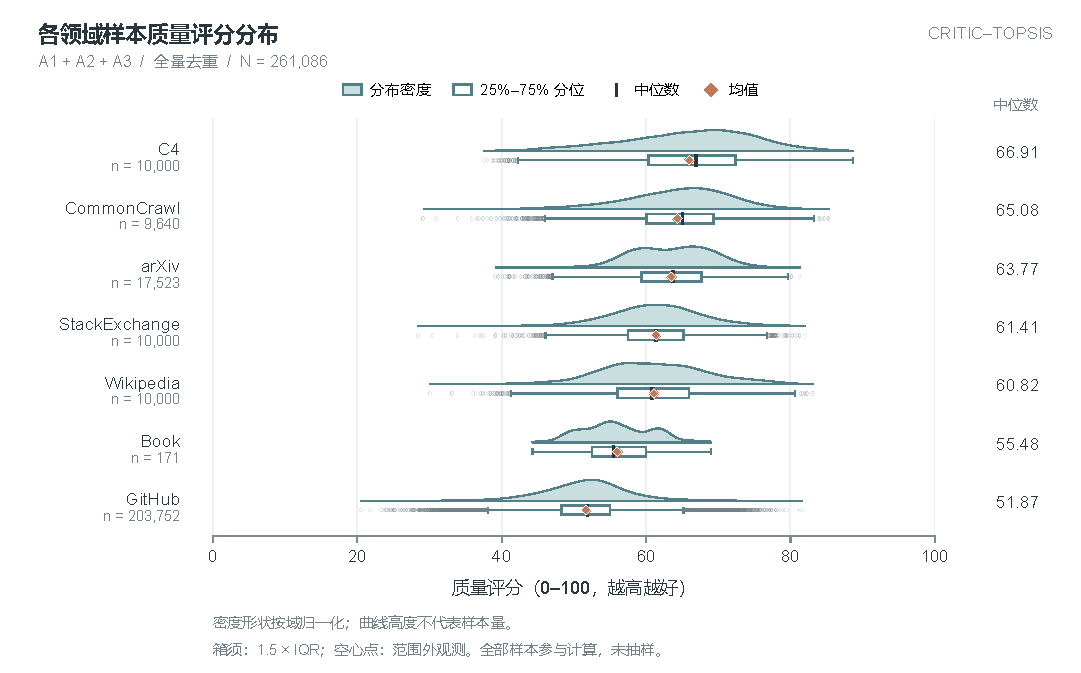
\includegraphics[width=\linewidth,height=0.42\textheight,keepaspectratio]{figures/q1-critic-topsis/nature-v1/figure01_domain_distribution_nature.pdf}
  \caption{领域质量分布图}
  \label{fig:q1-nature-01}
\end{figure}

\subsection{数据对象与预处理}
第 $i$ 条记录具有 16 维原始质量指标向量。指标覆盖语言形式、可读性、内容质量、教育性、事实性、知识覆盖与重复性等维度，其中句末标点率、cleanliness、no-ad、readability、fluency、unique words、QuRating education、writing、FineWeb education、factual、Books、Math 和 Wikipedia 为正向指标；无字母词比例、最高频二元词组占比和最高频三元词组占比为负向指标。负向指标较大时通常意味着文本更可能由符号、模板或高频短语主导，因此需要反向处理。
\formulaname{原始质量指标向量公式}
\begin{equation}
 \boldsymbol{x}_i=(x_{i1},\ldots,x_{i16}).
 \label{eq:q1-indicator-vector}
\end{equation}

正向与负向指标集合分别记为 $\mathcal P$、$\mathcal N$，两者互不相交且覆盖全部 16 个指标。方向统一后的指标定义如下。
\formulaname{指标方向统一公式}
\begin{equation}
 \widetilde{x}_{ij}=\begin{cases}
 x_{ij}, & j\in\mathcal{P},\\
 -x_{ij}, & j\in\mathcal{N}
 \end{cases}
 \label{eq:q1-direction-unification}
\end{equation}
随后使用方向统一值的 $A_1$ 拟合 $1\%$ 和 $99\%$ 分位点作为稳健边界；记边界为 $l_j$ 和 $u_j$，则统一为“越高越好”的稳健归一化形式。这里 $\operatorname{clip}(t,0,1)$ 表示将 $t$ 截断至 $[0,1]$。
\formulaname{稳健归一化公式}
\begin{equation}
 z_{ij}=\operatorname{clip}\left(\frac{\widetilde{x}_{ij}-l_j}{u_j-l_j},0,1\right).
 \label{eq:q1-robust-normalization}
\end{equation}
扩展集只使用 $A_1$ 的边界，不重新拟合分位点，从而保证 $A_1$、$A_2$ 和 $A_3$ 的分数具有可比性。归一化后检查缺失值、无穷值、越界值和重复指纹，并保留每条记录的来源集、领域标签和质量分数，供后续聚合与审计。

\begin{figure}[htbp]
  \centering
  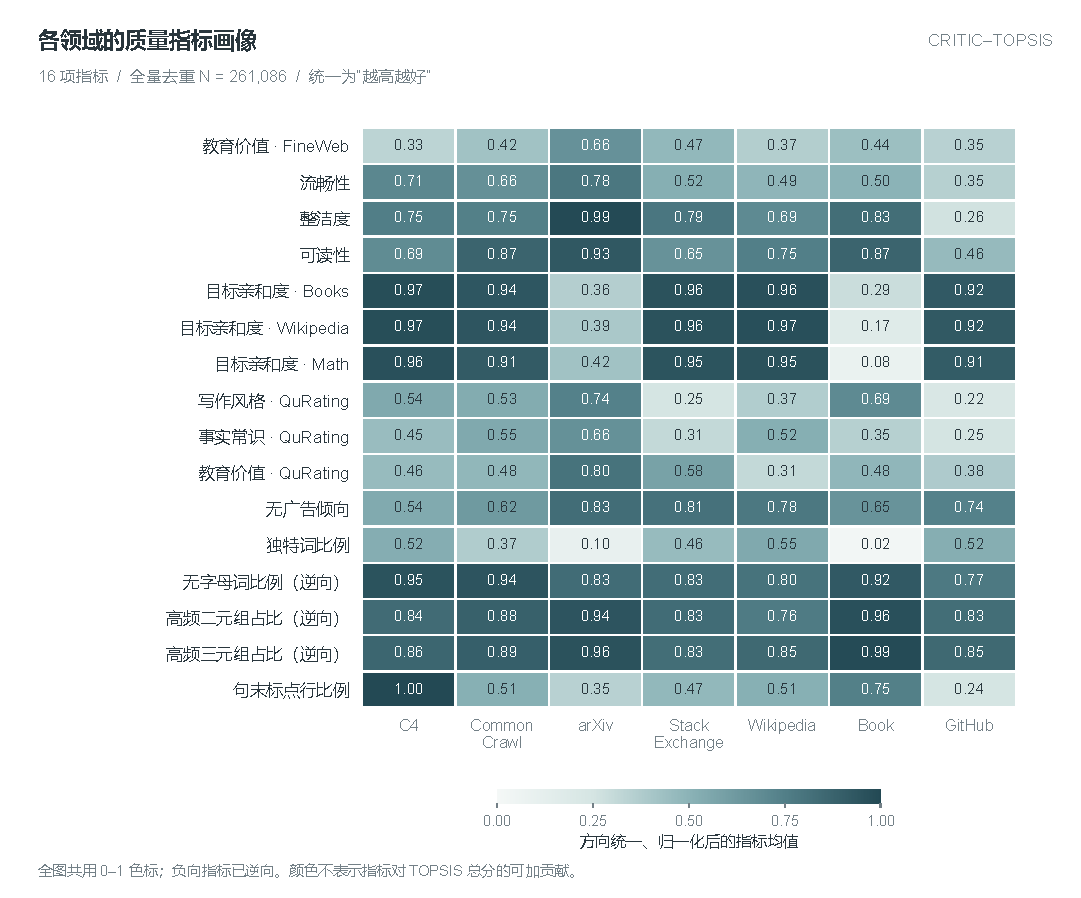
\includegraphics[width=\linewidth,height=0.42\textheight,keepaspectratio]{figures/q1-critic-topsis/nature-v1/figure02_indicator_heatmap_nature.pdf}
  \caption{领域质量指标画像图}
  \label{fig:q1-nature-02}
\end{figure}

\subsection{CRITIC 客观赋权}
为避免人为指定权重，采用 CRITIC 方法同时利用指标的离散程度和冲突程度。设归一化矩阵为 $Z$，其元素为 $z_{ij}$；第 $j$ 个指标的标准差为 $\sigma_j$，与第 $k$ 个指标的 Pearson 相关系数为 $r_{jk}$。
\formulaname{CRITIC 信息量公式}
\begin{equation}
 I_j=\sigma_j\sum_{k=1}^{16}(1-r_{jk}).
 \label{eq:q1-critic-information}
\end{equation}
\formulaname{CRITIC 权重公式}
\begin{equation}
 w_j=\frac{I_j}{\sum_{m=1}^{16}I_m}.
 \label{eq:q1-critic}
\end{equation}
其中，$\sigma_j$ 反映指标对样本的区分能力，$1-r_{jk}$ 反映该指标与其他指标的信息差异。由 $A_1$ 的拟合集计算权重并固定应用于 $A_1$ 留出集及 $A_2$、$A_3$，既防止扩展集的分布变化改变权重，又保证外推比较的可重复性。最终权重最高的指标为句末标点率（$8.9093\%$）、cleanliness（$8.0008\%$）和 no-ad（$7.7530\%$）；三个负向词组指标合计权重为 $16.5784\%$。

\begin{figure}[htbp]
  \centering
  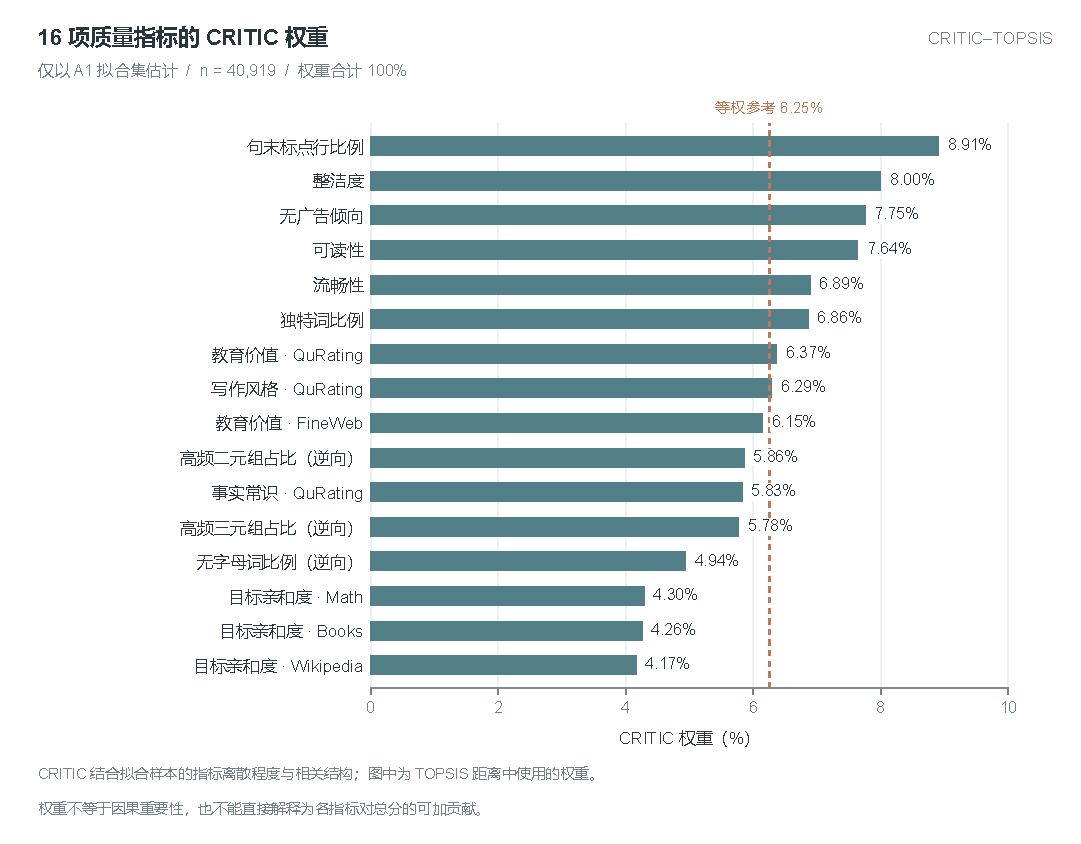
\includegraphics[width=\linewidth,height=0.42\textheight,keepaspectratio]{figures/q1-critic-topsis/nature-v1/figure05_critic_weights_nature.pdf}
  \caption{质量指标权重图}
  \label{fig:q1-nature-05}
\end{figure}

\subsection{加权距离 TOPSIS 评分}
以取值全为 1 的正向理想点 $\boldsymbol{z}^{+}$ 和取值全为 0 的负向理想点 $\boldsymbol{z}^{-}$ 为参照，计算第 $i$ 条记录到两类理想点的加权欧氏距离。
\formulaname{正理想点距离公式}
\begin{equation}
 D_i^{+}=\sqrt{\sum_{j=1}^{16}w_j(1-z_{ij})^2}.
 \label{eq:q1-topsis-positive-distance}
\end{equation}
\formulaname{负理想点距离公式}
\begin{equation}
 D_i^{-}=\sqrt{\sum_{j=1}^{16}w_jz_{ij}^2}.
 \label{eq:q1-topsis-distance}
\end{equation}
样本级质量分数定义如下，其取值在 $[0,100]$。
\formulaname{样本质量分数公式}
\begin{equation}
 Q_i=100\times\frac{D_i^{-}}{D_i^{+}+D_i^{-}}.
 \label{eq:q1-topsis-score}
\end{equation}
因此，$Q_i$ 越大表示该记录越接近理想高质量点。该分数回答的是“单条文本在 16 个统一方向质量信号下的综合质量水平”，而非某个单一指标的原始测量值。

\begin{figure}[htbp]
  \centering
  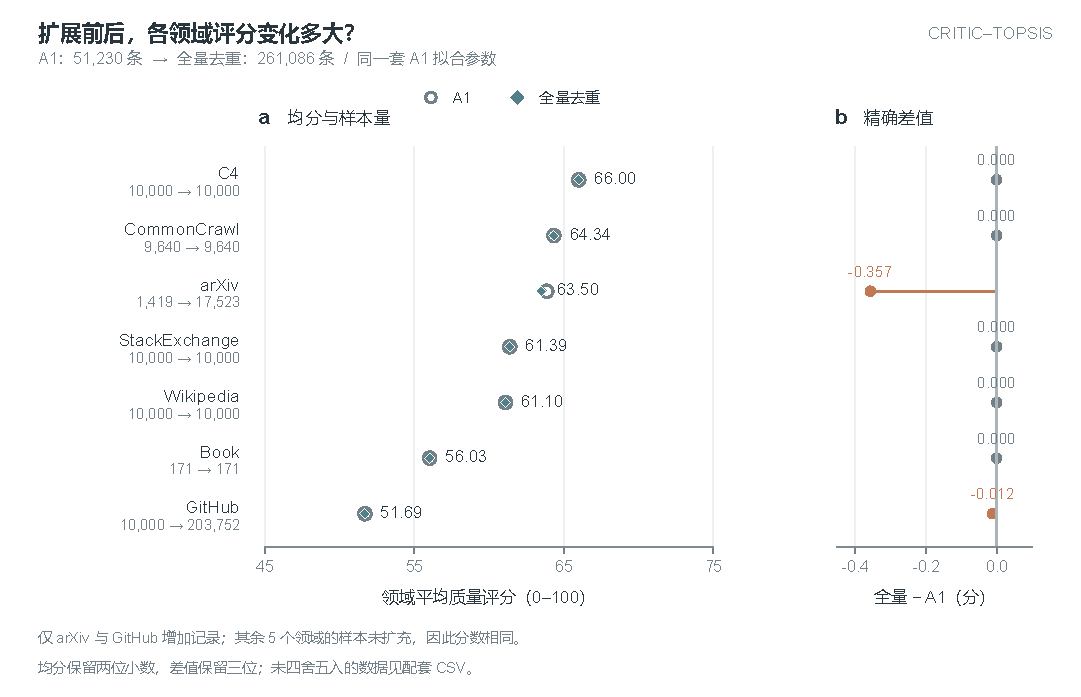
\includegraphics[width=\linewidth,height=0.42\textheight,keepaspectratio]{figures/q1-critic-topsis/nature-v1/figure03_A1_full_comparison_nature.pdf}
  \caption{领域均分对照图}
  \label{fig:q1-nature-03}
\end{figure}

\subsection{从样本级到领域级和语料级的聚合}
对领域 $g$ 的记录集合 $\mathcal{I}_g$，采用样本数加权的均值聚合。
\formulaname{领域质量均值公式}
\begin{equation}
 Q_g=\frac{1}{|\mathcal{I}_g|}\sum_{i\in\mathcal{I}_g}Q_i.
 \label{eq:q1-domain-aggregation}
\end{equation}
语料级分数同样由全体记录的样本均值给出。这种聚合保留了每条记录的等贡献原则，并能将域级差异与域规模分离：域均值反映质量，域记录数反映组成。若需降低极端值影响，可在附录中同时报告中位数和四分位距，但主结果使用均值以便与全量语料平均质量一致。
\formulaname{语料质量均值公式}
\begin{equation}
 Q_{\mathrm{corpus}}=\frac{1}{N}\sum_{i=1}^{N}Q_i.
 \label{eq:q1-corpus-aggregation}
\end{equation}

\begin{figure}[htbp]
  \centering
  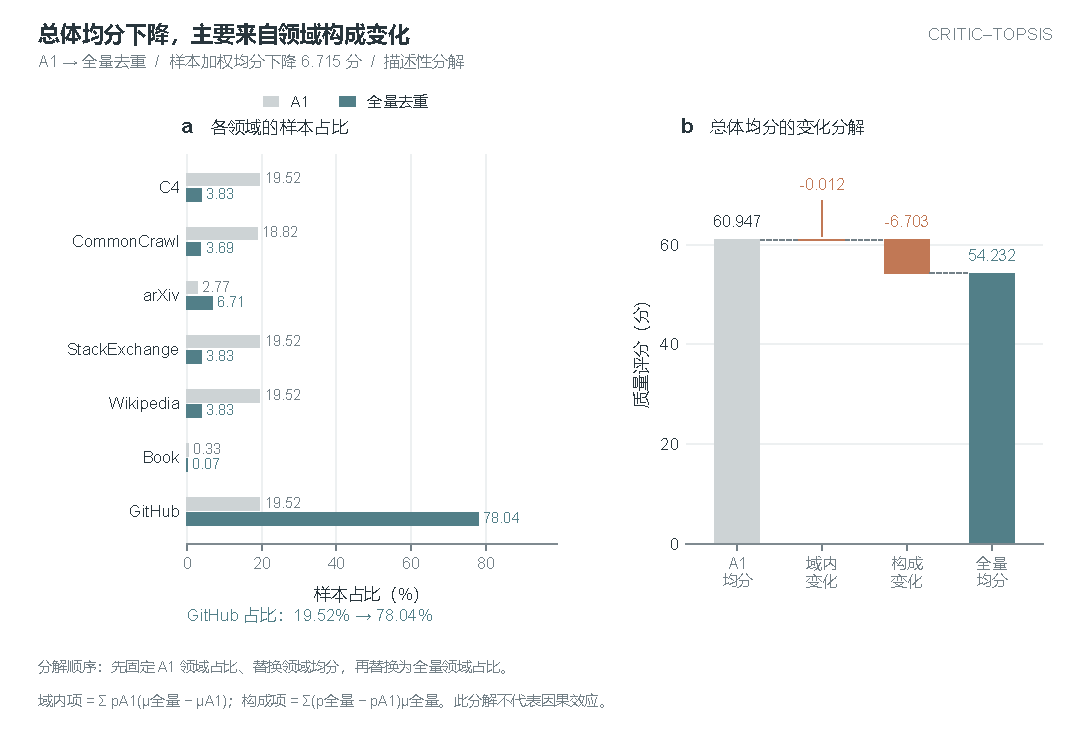
\includegraphics[width=\linewidth,height=0.42\textheight,keepaspectratio]{figures/q1-critic-topsis/nature-v1/figure04_composition_decomposition_nature.pdf}
  \caption{领域构成分解图}
  \label{fig:q1-nature-04}
\end{figure}

\subsection{全量结果与抽样集对照}
$A_1$ 语料级平均分为 $60.9471$，全量去重语料平均分为 $54.2323$，整体下降 $6.7149$ 分。按领域对照时，arxiv 从 $63.8624$ 变为 $63.5050$，下降 $0.3574$ 分；github 从 $51.7014$ 变为 $51.6893$，下降 $0.0121$ 分；book、c4、commoncrawl、stackexchange 和 wikipedia 的领域均值保持不变或仅发生四舍五入范围内的变化。由此可见，全量平均分下降主要来自领域组成变化，而不是各领域内部质量普遍恶化。GitHub 在 $A_1$ 中约占 $19.52\%$，在全量去重语料中约占 $78.04\%$，其较低的领域均值显著拉低了全量语料级分数。

\begin{table}[htbp]
  \centering
  \caption{$A_1$ 与全量去重语料的领域级质量分数对照}
  \label{tab:q1-domain-score}

  \renewcommand{\arraystretch}{1.15}
  \begin{tabular}{lrrrr}
    \toprule
    领域 & $A_1$ 均值 & 全量均值 & 变化 & 全量占比 \\
    \midrule
    arxiv & 63.8624 & 63.5050 & -0.3574 & 6.71\% \\
    book & 56.0325 & 56.0325 & 0.0000 & 0.07\% \\
    c4 & 66.0021 & 66.0021 & 0.0000 & 3.83\% \\
    commoncrawl & 64.3357 & 64.3357 & 0.0000 & 3.69\% \\
    github & 51.7014 & 51.6893 & -0.0121 & 78.04\% \\
    stackexchange & 61.3879 & 61.3879 & 0.0000 & 3.83\% \\
    wikipedia & 61.1009 & 61.1009 & 0.0000 & 3.83\% \\
    \addlinespace[0.5ex]
    语料级均值 & 60.9471 & 54.2323 & -6.7149 & 100.00\% \\
    \bottomrule
  \end{tabular}
\end{table}

\subsection{稳健性与适用边界}
将 CRITIC--TOPSIS 结果与等权加权、删除 DSIR 以及删除三个负向词组指标的敏感性方案比较。CRITIC 加权和等权结果的 Spearman 相关系数为 $0.9877$，CRITIC 结果与删除 DSIR 的结果相关系数为 $0.9860$，与删除三个负向指标的结果相关系数为 $0.9674$。在删除负向指标的方案中，平均名次变化为 $4.79$ 个百分点，约 $2.78\%$ 的记录名次变化超过 $20$ 个百分点，说明重复性指标虽不是唯一质量依据，但对尾部样本的排序具有实质影响。这里的敏感性分析用于检查第一小问质量评分对建模选择的稳定性；它不等同于问题一后续小问中对指标冲突的独立量化。

\begin{figure}[htbp]
  \centering
  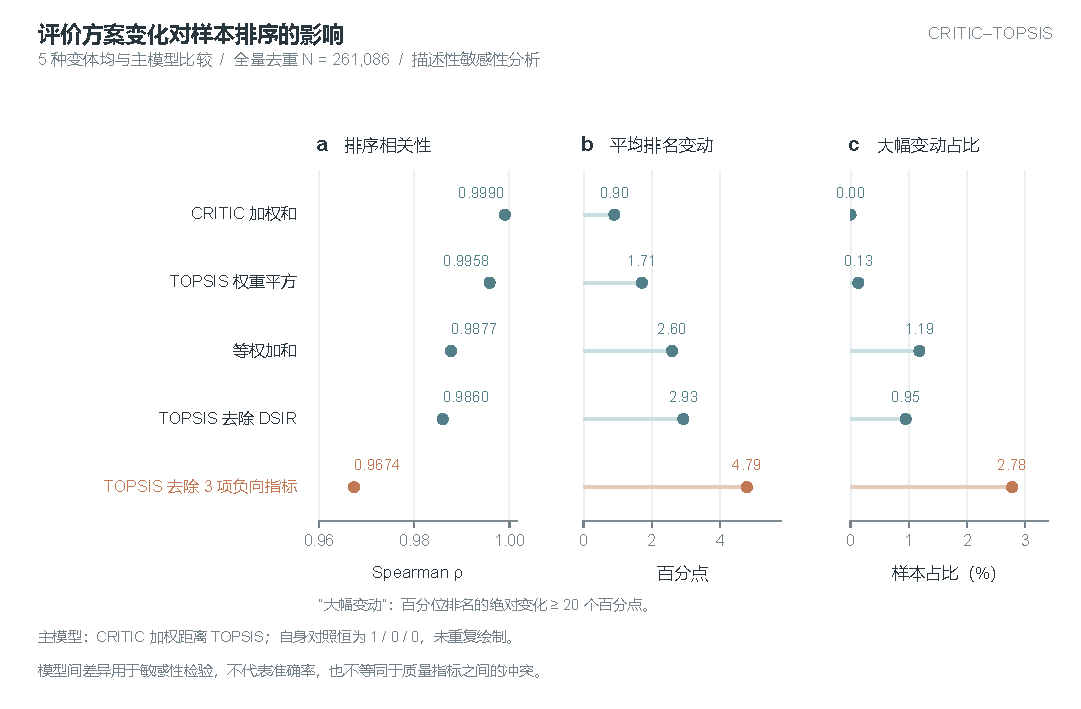
\includegraphics[width=\linewidth,height=0.42\textheight,keepaspectratio]{figures/q1-critic-topsis/nature-v1/figure06_model_sensitivity_nature.pdf}
  \caption{评分排序敏感性图}
  \label{fig:q1-nature-06}
\end{figure}

\subsection{小结}
本小问形成了一个可复算的全量质量评价链条：以 $A_1$ 的稳健边界和 CRITIC 权重建立统一标尺，以加权距离 TOPSIS 输出样本级质量分数，再按记录均值聚合为领域级和语料级分数。结果表明，$A_1$ 与扩展后的全量语料在领域内部质量上总体稳定，语料级平均分的主要变化由领域配比改变所致。该结论为后续质量冲突识别和数据配比优化提供可追溯的基线。

\FloatBarrier

\section{问题一：质量冲突消解与综合评价模型}
\label{sec:q12}

\subsection{文献依据与模型选择}

多指标评价的冲突可能来自同一属性的测量分歧，也可能来自不同属性之间的取舍。文献的部分研究决策研究采用极小极大方法协调冲突\cite{yu2016}；部分研究强调辨别冲突信息的来源，再确定融合权重\cite{wang2023}；部分研究将冲突测度与决策目标相联系\cite{chen2026}。这些研究对象不同于文本质量，但共同表明冲突分型应先于聚合规则的选择。

第一小问采用的 CRITIC 权重由指标离散度及相关性确定\cite{diakoulaki1995}，然而本题中的“指标冲突”描述的是样本间统计关系而非只关乎权重。并且存在于同一个文本中存在一个评价方向高分而另一个评价方向低分，故采用加权平均来用高分弥补低分，其补偿程度需单独建模\cite{giarlotta2001}。FineWeb 和 DataComp-LM 的实验表明数据过滤方式会影响语言模型表现\cite{penedo2024,li2024}。因而保留原 CRITIC--TOPSIS 分数，另构造冲突标记与有限补偿评价分。

\subsection{数据衔接与冲突定义}

设 $x_{ij}\in[0,1]$ 为方向统一后的第 $j$ 项指标，$w_j\geq0$ 为第一小问权重。把 11 项较通用指标归为五组 $G_g$：内容价值、表达质量、整洁度、无广告程度和非重复程度。组内均分与组权重定义为：
\begin{equation}
z_{ig}=\frac{\sum_{j\in G_g}w_jx_{ij}}{\sum_{j\in G_g}w_j},\qquad
v_g=\frac{\sum_{j\in G_g}w_j}{\sum_{h=1}^{5}\sum_{j\in G_h}w_j},
\qquad \sum_{g=1}^{5}v_g=1.
\label{eq:q12-group}
\end{equation}

内容价值包括 FineWeb 教育价值、QuRating 教育价值及事实与常识代理。表达质量包括英语流畅度、可读性及写作风格；非重复程度包括独特词比例及两项反向高频词组指标；第一小问原评分及全指标对照中仍保留DSIR 三项、无字母词比例和句末标点比例。

在 A1 拟合集计算并选定每组的 $20\%$ 与 $80\%$ 分位阈值 $l_g,h_g$。定义高低集合与冲突标记：
\begin{equation}
H_i=\{g:z_{ig}>h_g\},\qquad
L_i=\{g:z_{ig}<l_g\},\qquad
I_i=\mathbf{1}\{|H_i|>0\ \land\ |L_i|>0\}.
\label{eq:q12-conflict}
\end{equation}

严格不等号使处于阈值上的样本归入中间状态。$I_i=1$ 只表示同一文本至少有一组相对突出、另一组相对偏低。由 $H_i,L_i$ 表示是否为空，可得到冲突、仅优势、仅短板、中间状态四个互斥且穷尽的类别。冲突程度定义为：
\begin{equation}
C_i=\max_g\left[\frac{z_{ig}-h_g}{1-h_g}\right]_+
    \max_g\left[\frac{l_g-z_{ig}}{l_g}\right]_+,
\qquad
B_i=\frac{|H_i||L_i|}{\binom{5}{2}}.
\label{eq:q12-strength}
\end{equation}
其中 $C_i$ 为跨阈幅度，$B_i$ 为高低组配对广度。阈值来自 A1 拟合集，数值见表~\ref{tab:q12-thresholds}。

\begin{table}[htbp]
\centering
\caption{五维冲突判别阈值与权重}
\label{tab:q12-thresholds}
\begin{tabular}{lccc}
\toprule
维度 & 低阈值 $l_g$ & 高阈值 $h_g$ & 组权重 $v_g$ \\
\midrule
内容价值   & 0.2783 & 0.5613 & 0.2499 \\
表达质量   & 0.3578 & 0.7702 & 0.2836 \\
整洁度     & 0.2673 & 0.9884 & 0.1090 \\
无广告程度 & 0.5244 & 0.9004 & 0.1056 \\
非重复程度 & 0.6366 & 0.7838 & 0.2519 \\
\bottomrule
\end{tabular}
\end{table}

\subsection{冲突成因与消解规则}

在选定的评价质量指标冲突情况归纳中存在三种不同类型冲突，且对于不同类型的冲突应采取不同处理。第一种冲突为\textbf{测量冲突}，如两种教育维度对同一属性展现出一高一低。第二种冲突为\textbf{属性权衡冲突}，如内容价值高并且广告信号强、整洁度高而非重复程度低，考虑通过限制不同维度的相互补偿表达决策偏好。第三种冲突\textbf{适用性冲突}，即代码、非英语和 LaTeX 文本的英语流畅度高但是格式分低。

A1 中两种教育评分一高一低的样本为 415 条（$0.8101\%$），全量去重样本中有 1,402 条（$0.5370\%$）；组内分歧可能被五维平均后被掩盖，需要分开分析。以内容价值高且无广告程度低判别，A1 命中 1,884 条；换成原始广告 logit 大于无广告 logit，仅有 310 条。15 条定向原文案例虽然揭示了上述可能机制，但不能估计总体误判率。

\subsection{有限补偿综合评价模型}

第一小问的原分 $Q_i^{(0)}$ 作为参照。为处理属性间权衡采用名义权重来计算，即采用五个维度的各组权重；计算方法采用先把同一组内的 CRITIC 指标权重相加，再除以五组所包含指标的权重总和所得到的权重。先构造五维加权平均 $M_i=\sum_gv_gz_{ig}$，再允许组权重在名义权重 $v$ 附近变化。令 $\Delta_5=\{p:p_g\geq0,\sum_gp_g=1\}$，定义：
\begin{equation}
\mathcal W_{\lambda}=\{(1-\lambda)v+\lambda p:p\in\Delta_5\},\qquad
Q_i^{\mathrm{rob}}(\lambda)=100\min_{a\in\mathcal W_{\lambda}}\sum_{g=1}^{5}a_gz_{ig},
\quad 0\leq\lambda\leq1.
\label{eq:q12-robust}
\end{equation}

$\lambda$ 是对组权重不确定性的保守程度。内层目标关于 $p$ 为线性函数，在单纯形顶点取得最小值，因此若 $m_i=\min_g z_{ig}$，便有闭式解：
\begin{equation}
Q_i^{\mathrm{rob}}(\lambda)=100\big[(1-\lambda)M_i+\lambda m_i\big],\qquad
Q_i^{\mathrm{rob}}(\lambda)-100M_i=-100\lambda(M_i-m_i).
\label{eq:q12-closed}
\end{equation}

$\lambda=0$ 是五维加权平均，$\lambda=1$ 是最弱维度；对任意 $0\leq\lambda\leq1$，有 $100m_i\leq Q_i^{\mathrm{rob}}\leq100M_i$。所有组值同为 $c$ 时，得分为 $100c$；任一组值上升而其余不变时，得分不会下降。为限制优势维度在五维中为薄弱维度过度补偿，从而无法在保留平均表现的情况下考虑最弱一项，我们采用以模型最弱维度限制优势维度的补偿，不修改原始指标的方式作为补偿规则，故而可以使连续评分避免样本刚跨过冲突阈值就突然扣分。取 $\lambda=0.25$ ，原 16 维 TOPSIS 的差别同时包含指标选择和聚合方式变化，只有相对于五维加权平均的式~\eqref{eq:q12-closed} 分差才考虑归于补偿规则。

\subsection{A1 与扩展集结果}

\begin{table}[htbp]
\centering
\caption{冲突覆盖情况}
\label{tab:q12-coverage}
\begin{tabular}{lrrr}
\toprule
分区 & 样本数 & 冲突数 & 冲突率（\%） \\
\midrule
A1 全量         & 51,230  & 15,124 & 29.5218 \\
A1 留出集       & 10,311  & 3,039  & 29.4734 \\
A2 新增         & 16,104  & 9,408  & 58.4203 \\
A3 新增         & 193,752 & 65,795 & 33.9584 \\
A1--A3 唯一 ID & 261,086 & 90,327 & 34.5966 \\
\bottomrule
\end{tabular}
\end{table}

A1 四类样本数依次为 15,124、14,958、14,439、6,709，合计 51,230。拟合集冲突率 $29.5340\%$，留出集 $29.4734\%$，二者接近只说明本次划分下判别比例相近。arxiv 域在 A1 和新增集的冲突率分别为 $56.24\%$ 和 $58.42\%$；github 域分别为 $33.47\%$ 和 $33.96\%$。A2 新增中“整洁度高、非重复程度低”占 $54.53\%$，A3 新增中反向组合占 $26.27\%$，表明主要冲突模式随领域而变。其余五域没有扩展集可作同检验。把全量域级冲突率按 A1 领域比例重加权后为 $29.6680\%$，接近 A1 的 $29.5218\%$；总体率升至 $34.5966\%$ 主要与领域构成变化相关。图~\ref{fig:q12-pairs} 展示有向冲突组合，图~\ref{fig:q12-domain} 展示 A1 各领域差异，为量化质量信号冲突在不同领域中的分布差异，采用 A1 拟合集确定的统一分位阈值，将五个质量维度中同时存在高分与低分信号的文本标记为冲突，并统计各领域的冲突率及样本量。采用领域内比例有助于比较不同规模领域的冲突发生频率，同时报告样本量可以明确比例对应的数据基础。结果表明，A1 总体冲突率为$29.52\%$，各领域存在较大的描述性差异：arXiv 为 $56.24\%$，高于其他领域；StackExchange 为 $15.35\%$，相对较低。Book 的冲突率为 $46.78\%$。C4 的冲突率虽低于 arXiv，但其样本量较大，冲突数达到 3,939 条，为各领域最多。总体体现为，高低质量信号并存、频繁程度随领域而异。

同一文本可能计入多个高低分配对，如图~\ref{fig:q12-pairs} 中单元格所示。
\begin{figure}[htbp]
\centering
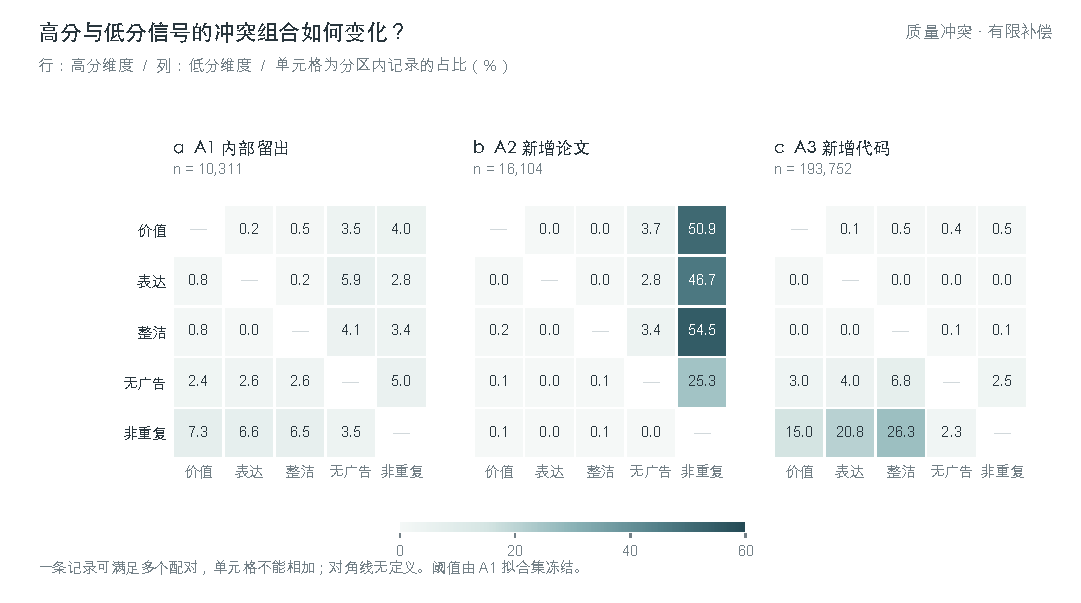
\includegraphics[width=\linewidth]{fig3_1_conflict_pair_heatmap.pdf}
\caption{高低分信号配对比例}
\label{fig:q12-pairs}
\end{figure}

\begin{figure}[htbp]
\centering
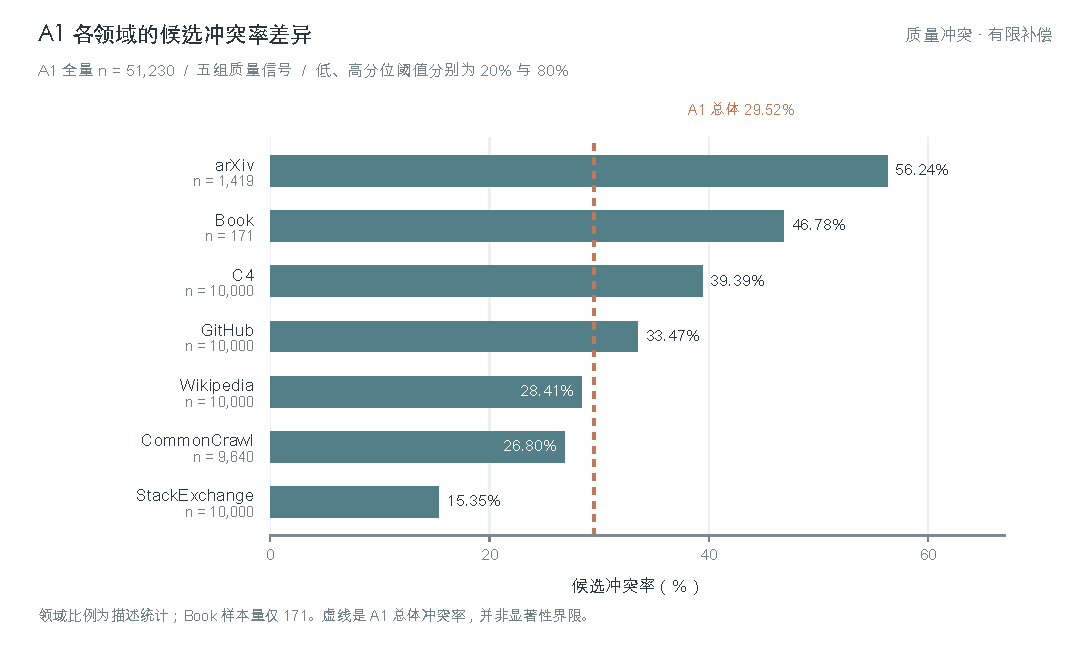
\includegraphics[width=0.92\linewidth]{fig3_2_domain_conflict.pdf}
\caption{A1 各领域冲突率及样本量}
\label{fig:q12-domain}
\end{figure}

\begin{table}[htbp]
\centering
\caption{均值分对比（下降量为模型规定的保守折减）}
\label{tab:q12-scores}
\begin{tabular}{lrrrr}
\toprule
分区 & 原 TOPSIS & 加权平均 & 有限补偿分 & 相对基线变化 \\
\midrule
A1 全量         & 60.9471 & 58.6944 & 52.8212 & $-5.8733$ \\
A1 留出集       & 61.0370 & 58.7548 & 52.8643 & $-5.8905$ \\
A2 新增         & 63.4735 & 76.5370 & 72.2455 & $-4.2915$ \\
A3 新增         & 51.6887 & 46.9338 & 40.4316 & $-6.5022$ \\
A1--A3 唯一 ID & 54.2323 & 51.0674 & 44.8250 & $-6.2424$ \\
\bottomrule
\end{tabular}
\end{table}

A2 新增有限补偿分与原 TOPSIS 分的 Spearman 相关为 0.6105，说明换指标与换聚合规则会明显改变排序。若将候选分作为后续配比或标度律输入，原质量评分与补偿风存在一定差异可能需要分别讨论。

\subsection{灵敏度、核验与适用边界}

图~\ref{fig:q12-threshold} 与图~\ref{fig:q12-lambda} 分别展示两类敏感性。第一种是冲突率对分位阙值的敏感性，见图可知把尾部分位从 $10\%$ 调至 $25\%$，A1 留出集冲突率由 $9.4074\%$ 升至 $41.4606\%$，A2 新增由 $3.8934\%$ 升至 $79.0673\%$，A3 新增由 $13.7919\%$ 升至 $44.2380\%$，冲突率高度依赖相对阈值，$\lambda$ 在 $0,0.1,0.25,0.5$ 上的变化影响候选均分。第二种是$\lambda$ 对候选均分的影响，~\eqref{eq:q12-closed} 还给出解析灵敏度 $\partial Q_i^{\mathrm{rob}}/\partial\lambda=-100(M_i-m_i)$，维度差距越大，保守程度的影响越强；最弱维度若受噪声或域失配影响，模型也会随之偏低。

\begin{figure}[htbp]
\centering
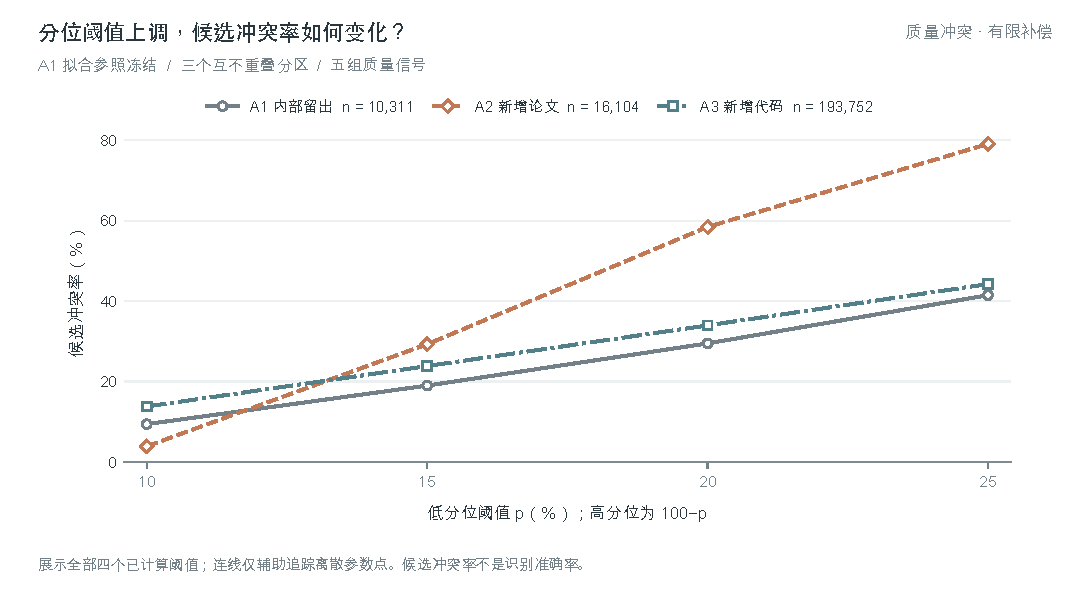
\includegraphics[width=0.92\linewidth]{fig3_3_threshold_sensitivity.pdf}
\caption{冲突率对分位阈值的敏感性}
\label{fig:q12-threshold}
\end{figure}

\begin{figure}[htbp]
\centering
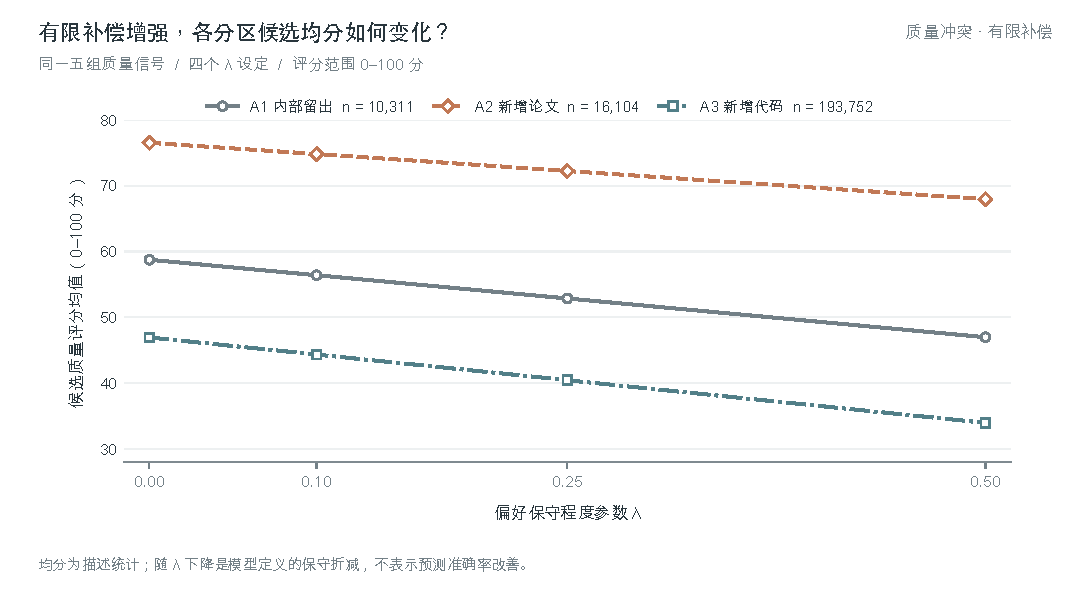
\includegraphics[width=0.92\linewidth]{fig3_4_compensation_sensitivity.pdf}
\caption{$\lambda$ 对均分的影响}
\label{fig:q12-lambda}
\end{figure}

原评分复算的七域均分最大误差小于 $10^{-12}$；重复 ID 的指标和领域一致，四类判别穷尽样本，式~\eqref{eq:q12-closed} 的闭式解与单调性可直接核对。



\FloatBarrier
% 问题一第三小问；依 main.tex 的 GMCMthesis 模板编译。
% 数据与图形源自 q1_s03_seven_figures；A12--A15 为给定估算 Loss。
\section{问题一：配比效应与规模修正}
\label{sec:q13}

第二小问通过冲突识别与有限补偿评分，给出了文本质量信号的审慎汇总方式；但评分的改变能否转化为语言模型收益，仍须由训练配方和验证 Loss 检验。为此，本小问以 17 个训练领域的配比向量 $\boldsymbol p_r$ 解释 13 个验证目标的 Loss，先估计同尺度的配比替代关系，再针对跨规模预测中的系统偏差进行修正。第二小问的候选质量分在此只作为可选代理参与增量对照，不预设其具有独立于配比的预测作用。

\subsection{配方结构与同尺度效应}

各配方满足非负及总和为 1 的约束。图~\ref{fig:q13-structure} 展示六组数据表的平均领域配比及三种不同实测配方设计的分布范围。A4/A5 含 512 个拟合配方，A6/A7 与 A8/A9 各含 256 个配方且二者配比相同；A10/A11 含 64 个配方，A12/A13 与 A14/A15 各含相同的 63 个配方。重复配方用于识别规模变化，不能增加独立的配方设计数。A10 在部分领域的配比范围与 A4 不同，因此后续领域替代效应只在非负且处于 A4 逐列边际范围内的配方上计算。

\begin{figure}[htbp]
  \centering
  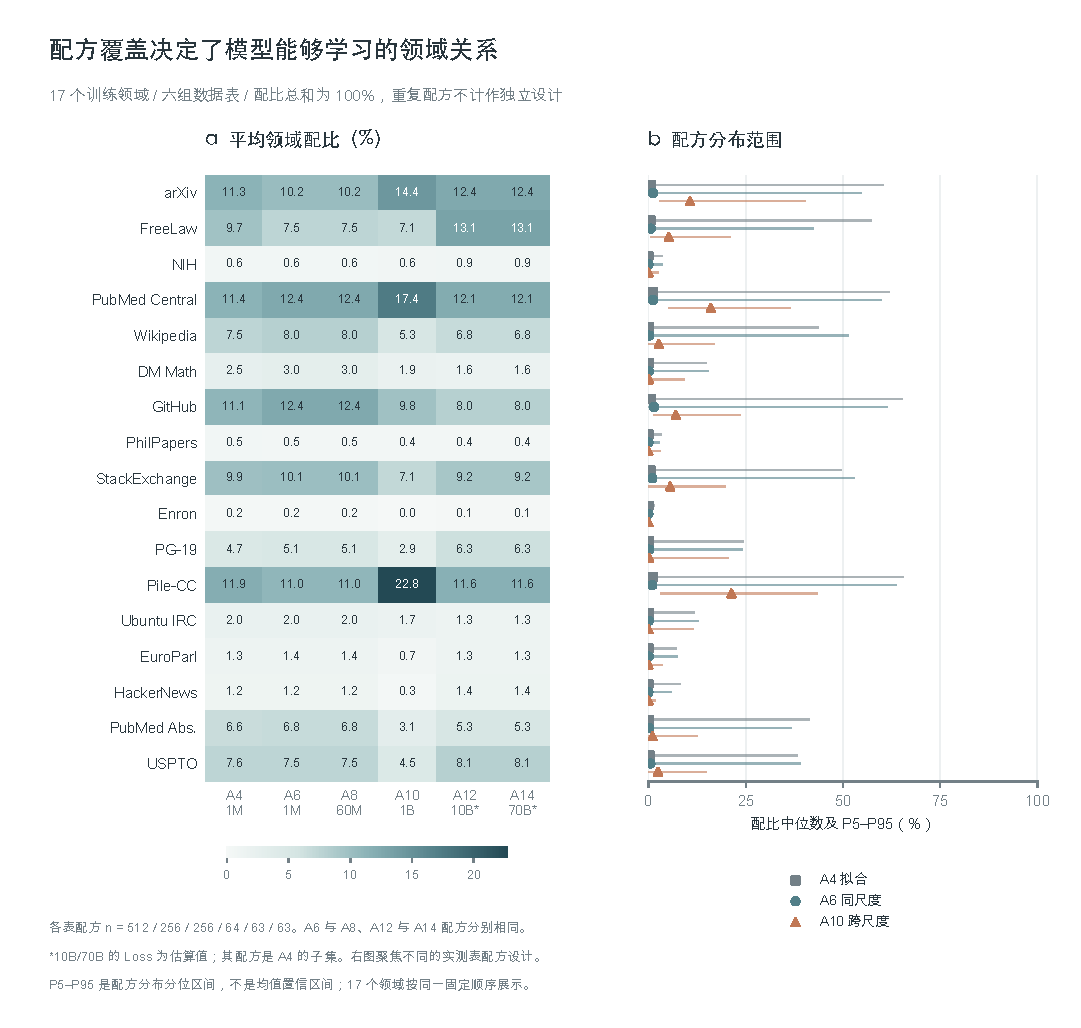
\includegraphics[width=\linewidth,height=0.65\textheight,keepaspectratio]{Fig01_recipe_structure.pdf}
  \caption{训练领域配比图}
  \label{fig:q13-structure}
\end{figure}

考虑到配比的闭合约束，模型对配比作等距对数比（ilr）变换，并以多响应 Ridge 回归刻画 13 个目标的 Loss。线性模型提供可解释基线，二阶模型容纳配比之间的非线性关系。为解释替代而非单独改变某一领域，固定从领域 $j$ 向领域 $i$ 转移一个百分点的配比，对合法配方计算模型预测差。
\formulaname{领域配比替代效应公式}

\begin{equation}
\Delta_{i\leftarrow j,k}(\boldsymbol p)=\hat L_k(\boldsymbol p+0.01\boldsymbol e_i-0.01\boldsymbol e_j)-\hat L_k(\boldsymbol p).\label{eq:q13-transfer}
\end{equation}

式中 $k$ 为验证目标，$\boldsymbol e_i$ 为第 $i$ 个单位向量；$\Delta<0$ 表示该目标的预测 Loss 降低。图~\ref{fig:q13-transfer} 对每个有向替代关系先在合法配方上求均值，再对 13 个目标等权平均。二阶模型的效应图较线性模型更具方向依赖性，提示配比组合会改变局部替代关系；但不同目标的正负效应可能在平均时抵消，图中颜色不能直接解释为因果效应或最优配方。

\begin{figure}[htbp]
  \centering
  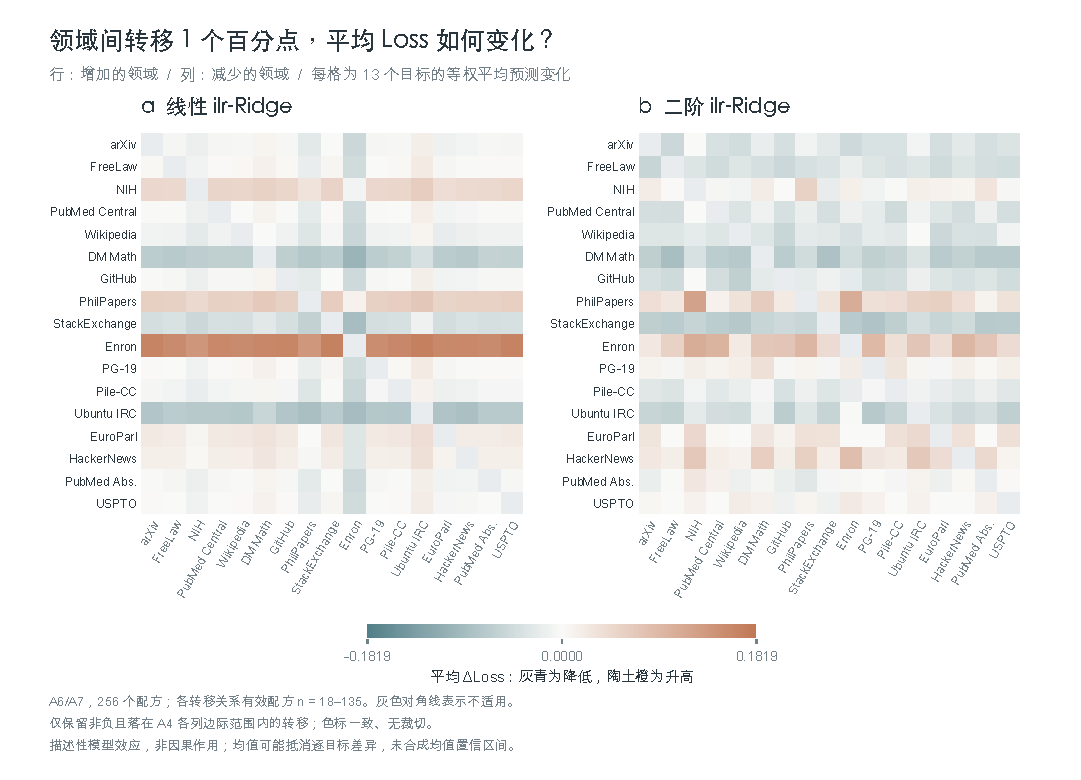
\includegraphics[width=\linewidth,height=0.58\textheight,keepaspectratio]{Fig02_domain_transfer.pdf}
  \caption{领域配比替代效应图}
  \label{fig:q13-transfer}
\end{figure}

同尺度检验支持保留二阶结构。图~\ref{fig:q13-stability}a、b 中，A6/A7 的 pooled RMSE 由线性模型的 0.3464 降至 0.2840，降幅为 18.0\%；MAE 由 0.2626 降至 0.2019，降幅为 23.1\%。按配方成对重采样得到的二阶减线性误差差值，RMSE 为 $-0.0624$（95\% 描述性区间 $[-0.0834,-0.0420]$），MAE 为 $-0.0607$（$[-0.0765,-0.0452]$）。这表明在固定模型条件下，非线性项确实改善了同尺度预测。图~\ref{fig:q13-stability}c 则使用较早的有限扰动运行：13 个目标、每目标 272 个有向替代关系的线性与二阶方向一致率大多约为 60\%--75\%。预测误差下降并不保证每一条领域替代解释稳定；该面板与前两面板来源不同，也不能视为最新模型的重复解释验证。

\begin{figure}[htbp]
  \centering
  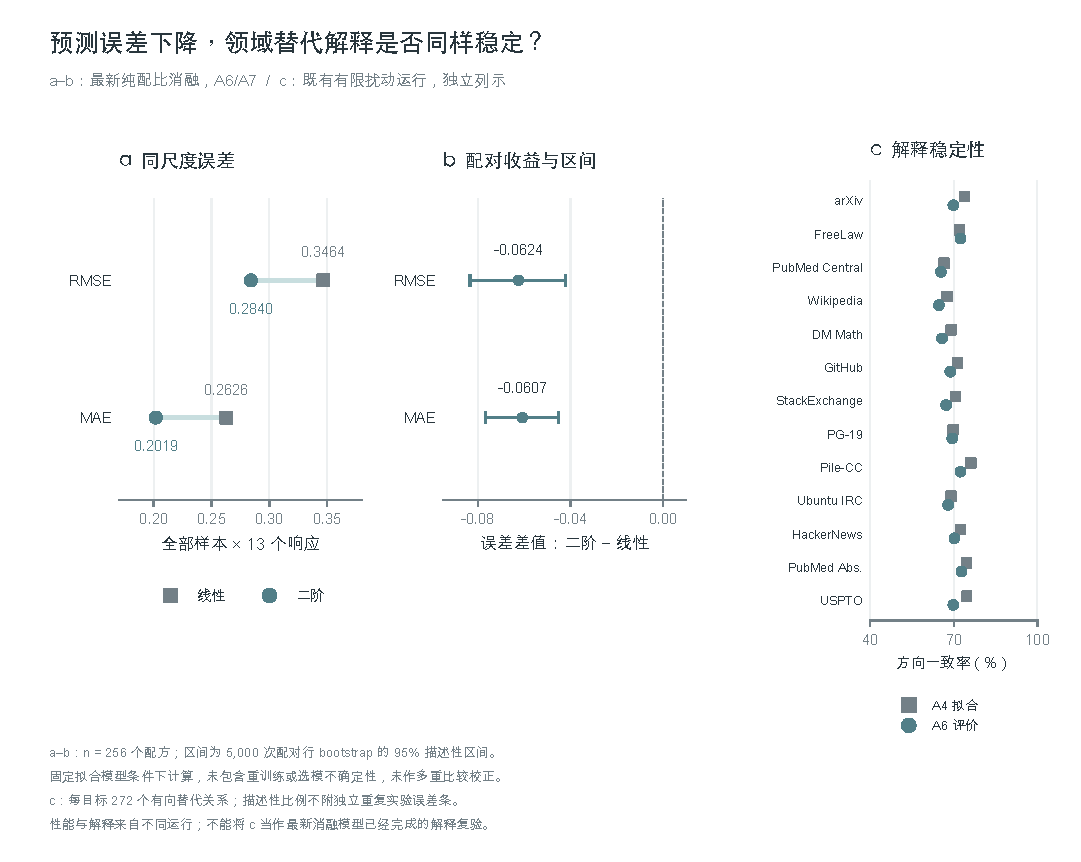
\includegraphics[width=\linewidth,height=0.56\textheight,keepaspectratio]{Fig03_prediction_and_stability.pdf}
  \caption{同尺度预测与稳定性图}
  \label{fig:q13-stability}
\end{figure}

\subsection{规模偏差的识别与修正收益}

仅以配比预测跨规模绝对 Loss 存在结构性遗漏：A6 与 A8 的配比逐行相同，而两表平均 Loss 相差 1.4594；同一配比的纯配比预测器只能给出同一个预测值。由此，将模型写为配比项与规模修正项之和，并要求修正项在 1M 基准尺度为零。
\formulaname{配比与规模联合预测公式}

\begin{equation}
\hat L_k(\boldsymbol p,S)=f_k\!\left[\operatorname{ilr}(\boldsymbol p)\right]+c_k(\boldsymbol p,S).\label{eq:q13-scale}
\end{equation}
\formulaname{基准规模约束公式}
\begin{equation}
c_k(\boldsymbol p,1\mathrm M)=0.\label{eq:q13-scale-baseline}
\end{equation}

比较的四种设置分别为无修正、全局修正、逐目标领域修正和配方条件修正。其共同依据是 A6/A7 与 A8/A9 的同配方跨规模差分；配方基础模型保持冻结，避免把规模偏移错误归入某个训练领域的系数。图~\ref{fig:q13-scale} 显示，二阶纯配比模型在 60M 表 A8/A9 的 pooled RMSE 为 1.5993，配方条件修正后为 0.3017；在 1B 表 A10/A11，该指标由 2.6963 降至 0.6252，降幅为 76.8\%。对应的 1B 逐目标平均 MAE 由 2.6203 降至 0.5207，降幅为 80.1\%。这说明显式处理规模偏差是跨尺度绝对误差下降的主要来源。然而，A8/A9 参与修正校准，A10/A11 也已多次用于回顾性比较；这些数字不构成独立的最终泛化精度。1B 的全局修正 MAE 为 0.4256，反而低于配方条件修正的 0.5207，说明更复杂的修正并非在所有指标上占优。

\begin{figure}[htbp]
  \centering
  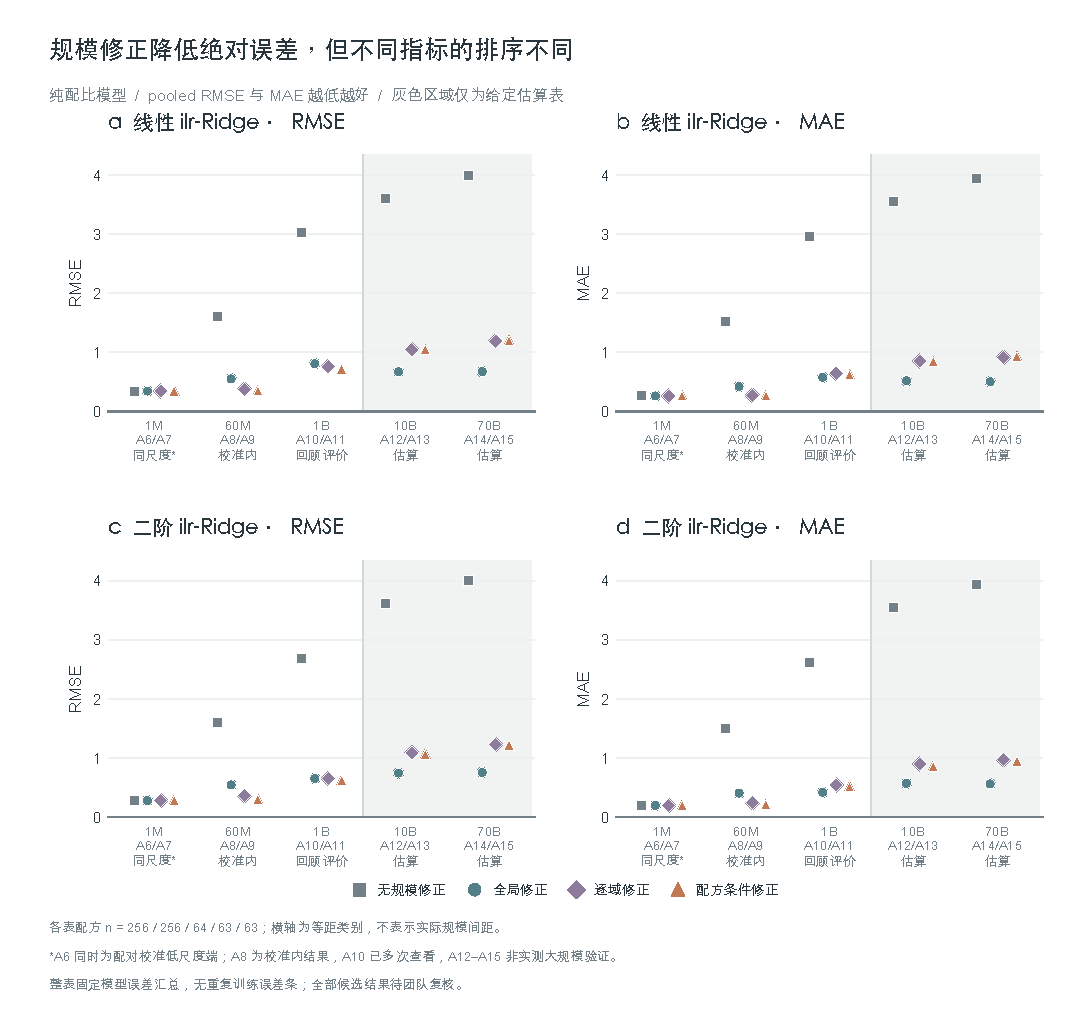
\includegraphics[width=\linewidth,height=0.65\textheight,keepaspectratio]{Fig04_scale_correction.pdf}
  \caption{规模修正误差图}
  \label{fig:q13-scale}
\end{figure}

为避免总体指标掩盖目标差异，图~\ref{fig:q13-targets}a、b 给出 1B 表中全部 13 个目标的 MAE 相对降幅。降幅按式~\eqref{eq:q13-reduction}计算，正值表示改善。
\formulaname{目标误差降幅公式}

\begin{equation}
R_{k,c}=\frac{\operatorname{MAE}_{k,0}-\operatorname{MAE}_{k,c}}{\operatorname{MAE}_{k,0}}\times100\%.\label{eq:q13-reduction}
\end{equation}

三类修正在两个基础模型的 13 个目标上均得到正降幅，但改善幅度不均，二阶模型下 DM Math 的全局修正降幅仅为 36.4\%，远低于 Pile-CC 的 97.7\%。图~\ref{fig:q13-targets}c 进一步揭示外推限制：同一批 63 个配方从 10B 到 70B 的给定平均 Loss 降幅为 0.3829，而三类修正预测降幅约为 0.6936、0.6936 和 0.6975，均明显偏大。规模修正解决了已观察到的大部分绝对偏移，却尚不能据估算表推出可靠的高规模尺度律。

\begin{figure}[htbp]
  \centering
  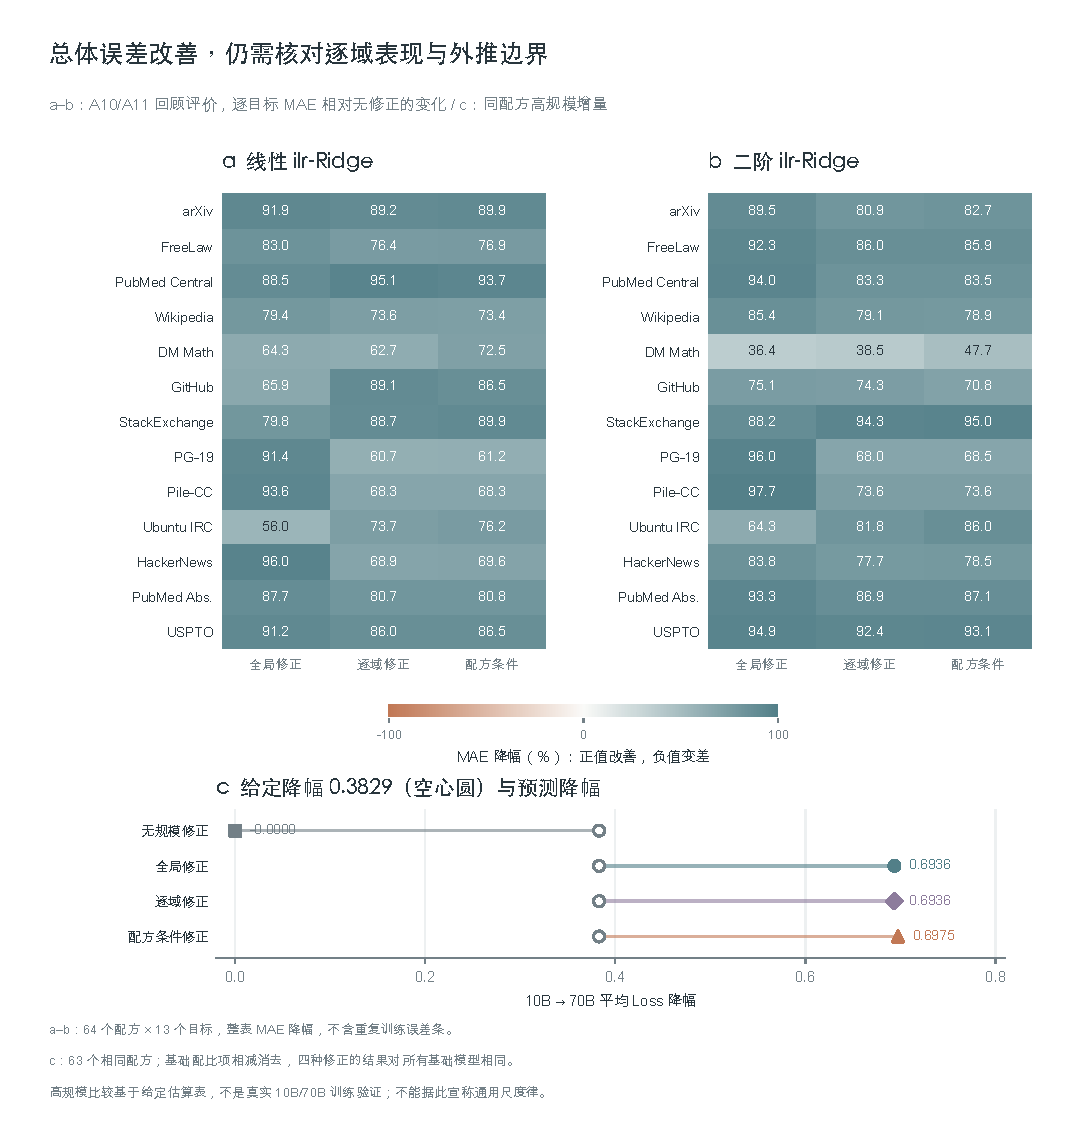
\includegraphics[width=\linewidth,height=0.68\textheight,keepaspectratio]{Fig05_domain_errors_and_extrapolation.pdf}
  \caption{目标误差与外推图}
  \label{fig:q13-targets}
\end{figure}

\subsection{补充诊断与模型边界}

第二小问的质量分提供了有意义的候选信息，但当前实验中的 $Q_{\mathrm{proxy}}$ 是配比的确定函数，并非独立观测到的文本质量。补充图~\ref{fig:q13-quality} 完整列出两类基础模型、四类修正和五组评价表的加入前后对照：在线性模型的 1M 同尺度评价中，加入代理后 RMSE 约下降 1.8\%；二阶模型在同一评价中的误差差值接近零且区间跨零，在部分跨尺度设置下还会变差。因此，现有结果不能把第二小问的评分修正表述为已被下游 Loss 验证的独立收益，更不能据此为质量代理赋予唯一因果系数。

\FloatBarrier
\subsection*{补充诊断图}
\setcounter{figure}{0}
\renewcommand{\thefigure}{S\arabic{figure}}
\begin{figure}[htbp]
  \centering
  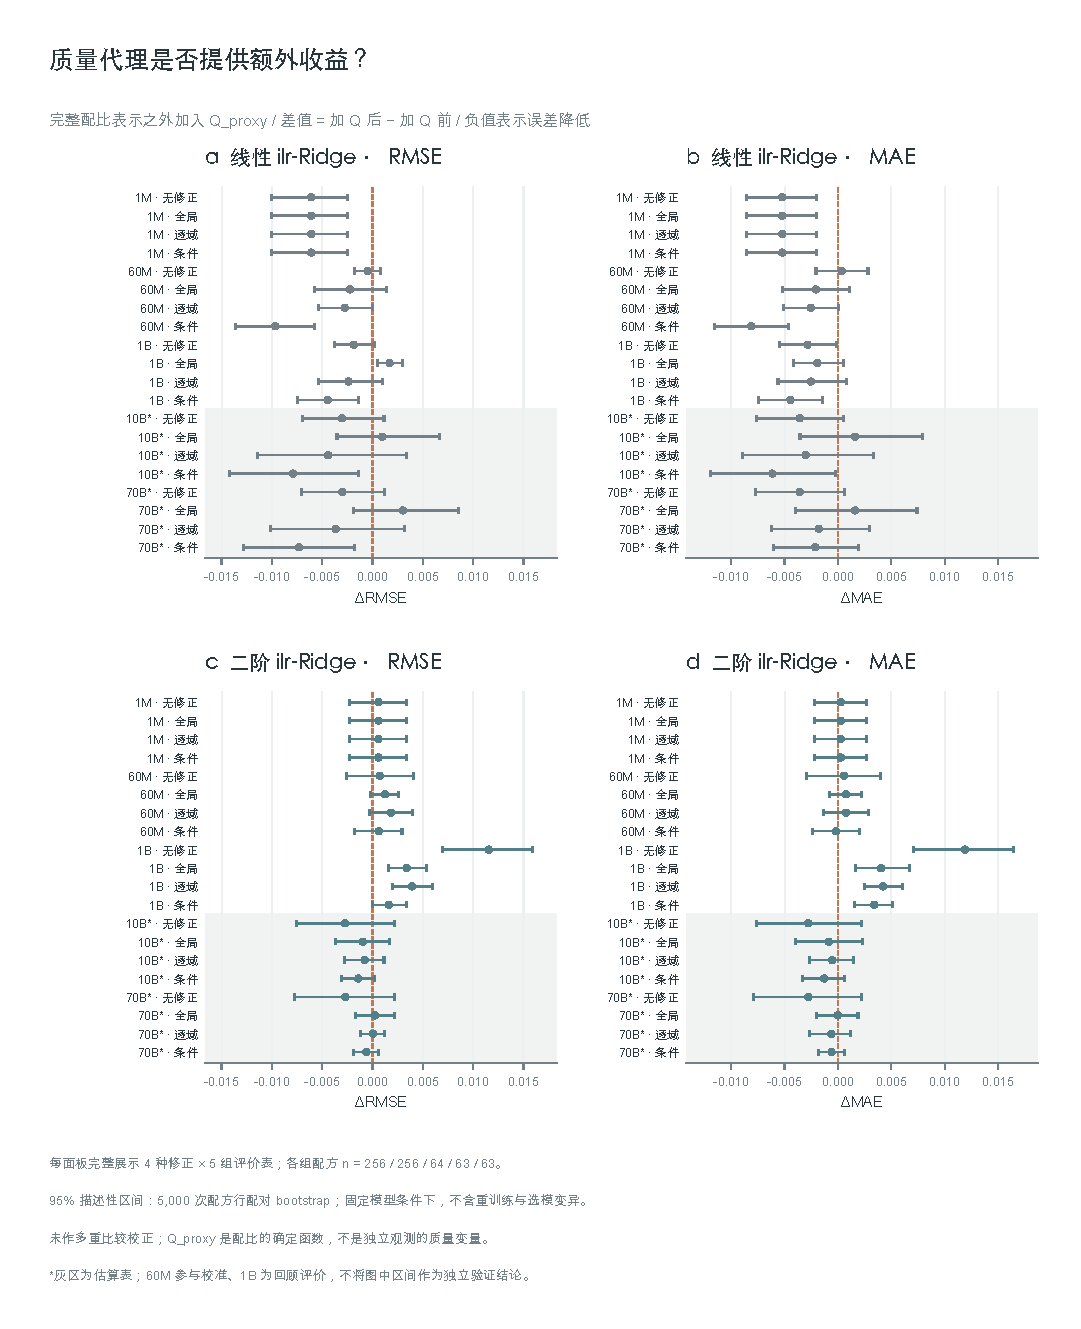
\includegraphics[width=\linewidth,height=0.82\textheight,keepaspectratio]{FigS01_optional_quality.pdf}
  \caption{质量代理增量图}
  \label{fig:q13-quality}
\end{figure}

补充图~\ref{fig:q13-oof} 使用 A8/A9 的 256 对配方，以完整配方对为单位分为五折，仅在训练折重拟合规模修正，配比基础模型保持冻结。二阶配方条件修正的 pooled RMSE 从校准内 0.3017 变为折外 0.3073，MAE 从 0.2128 变为 0.2157；折外误差仅小幅上升，说明此校准诊断中修正收益不完全依赖本配方参与拟合。但正则化系数沿用历史选择，且折外检验仍发生在参与规模校准的 60M 设计内，不能替代新规模、新配方的独立验证。

\begin{figure}[htbp]
  \centering
  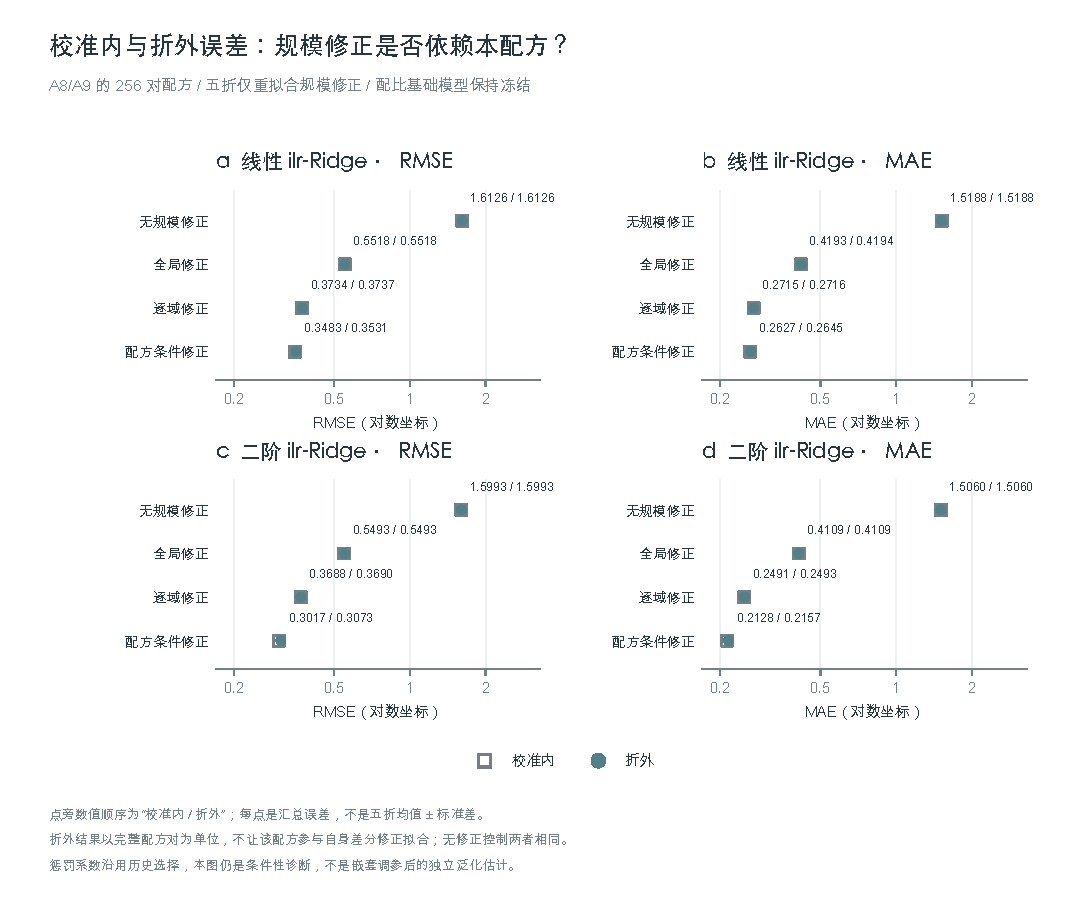
\includegraphics[width=\linewidth,height=0.62\textheight,keepaspectratio]{FigS02_calibration_oof.pdf}
  \caption{规模修正折外检验图}
  \label{fig:q13-oof}
\end{figure}

据此，第三小问的可支持结论是：同尺度配比关系存在可预测的非线性信号；同配方跨规模 Loss 差异要求显式规模修正；该修正在回顾性跨尺度评价中大幅降低绝对误差。领域替代关系仍是受配方支持范围约束的模型关联，高规模估算与质量代理的增量效果也尚不足以支持最优配方或通用尺度律的断言。

\FloatBarrier
% 全文参考文献；从问题一冲突消解章节移出，以便在各问正文后统一排版。
\begin{thebibliography}{99}
\bibitem{diakoulaki1995} DIAKOULAKI D, MAVROTAS G, PAPAYANNAKIS L. Determining objective weights in multiple criteria problems: The CRITIC method[J]. Computers \& Operations Research, 1995, 22(7): 763--770. DOI: \href{https://doi.org/10.1016/0305-0548(94)00059-H}{10.1016/0305-0548(94)00059-H}.
\bibitem{giarlotta2001} GIARLOTTA A. Multicriteria compensability analysis[J]. European Journal of Operational Research, 2001, 133(1): 190--209. DOI: \href{https://doi.org/10.1016/S0377-2217(00)00198-3}{10.1016/S0377-2217(00)00198-3}.
\bibitem{yu2016} 余高锋, 李登峰, 邱锦明, 等. 考虑偏好冲突的多类评价信息群体决策方法[J]. 控制与决策, 2016, 31(11): 2013--2018. DOI: \href{https://doi.org/10.13195/j.kzyjc.2015.0948}{10.13195/j.kzyjc.2015.0948}.
\bibitem{wang2023} 王雷, 王晓玲, 张君, 等. 考虑融合权重优化与冲突信息来源的大坝安全综合评价方法[J]. 清华大学学报(自然科学版), 2023, 63(10): 1566--1575. DOI: \href{https://doi.org/10.16511/j.cnki.qhdxxb.2023.22.039}{10.16511/j.cnki.qhdxxb.2023.22.039}.
\bibitem{chen2026} 陈雪龙, 王子睿, 李苗苗. 多周期应急资源调配主体冲突消解方法研究[J]. 中国管理科学, 2026, 34(3): 226--241. DOI: \href{https://doi.org/10.16381/j.cnki.issn1003-207x.2023.2186}{10.16381/j.cnki.issn1003-207x.2023.2186}.
\bibitem{penedo2024} PENEDO G, KYDLÍČEK H, BEN ALLAL L, et al. The FineWeb datasets: Decanting the web for the finest text data at scale[EB/OL]. 2024. \url{https://arxiv.org/abs/2406.17557}.
\bibitem{li2024} LI J, FANG A, SMYRNIS G, et al. DataComp-LM: In search of the next generation of training sets for language models[C]//Advances in Neural Information Processing Systems. 2024. \url{https://arxiv.org/abs/2406.11794}.
\end{thebibliography}


\end{document}
